\title{Introduzione alle Simulazioni di Dinamica Molecolare}
\author{
        Antonio Michele Miti \\
	Mat: 072838
%                Dipartimento di Fisica \\
%        Università Milano-Bicocca\\
%        Piazza della Scienza 3, Milano 20126, \underline{Italy}
}
%\date{\today}

% Formato pagina!
\documentclass[11pt]{article}
%\documentclass{acmconf}
\usepackage[paper=a4paper,dvips,top=1.5cm,left=1.5cm,right=1.5cm,
    foot=1cm,bottom=1.5cm]{geometry}

% Convenzioni Italiane
\usepackage[italian]{babel}



\usepackage{amsmath}

%Teoremi
\usepackage{amsthm}
\theoremstyle{plain}
\newtheorem{thm}{Teorema}[section]
\theoremstyle{remark}
\newtheorem{oss}{Osservazione}

%campi numerici
\usepackage{amsfonts}
\newcommand\Naturals{\ensuremath{\mathbb{N}}\xspace}
\newcommand\Integers{\ensuremath{\mathbb{Z}}\xspace}
\newcommand\Rationals{\ensuremath{\mathbb{Q}}\xspace}
\newcommand\Reals{\ensuremath{\mathbb{R}}\xspace}
\newcommand\Complex{\ensuremath{\mathbb{C}}\xspace}


%c C plus plus
\usepackage{relsize}
\usepackage{lipsum}
%c from texinfo.tex
\def\ifmonospace{\ifdim\fontdimen3\font=0pt }
\def\C++{%
\ifmonospace%
    C++%
\else%
    C\kern-.1667em\raise.30ex\hbox{\smaller{++}}%
\fi%
\spacefactor1000 }
%caratteri personalizzati per c++
\newcommand\Cls[1]{\textsf{#1}}
\newcommand\Lang[1]{\textsc{#1}}
\newcommand{\kw}[1]{\texttt{\textbf{#1}}}
\newcommand{\cd}[1]{\texttt{#1}}


%lettere accentate
\usepackage[utf8]{inputenc}


%usare immagini
\usepackage{graphicx}
\usepackage{latexsym}
\usepackage{wrapfig}
\usepackage{epstopdf}
\usepackage{caption}
\usepackage{subcaption}
\usepackage{sidecap}
\usepackage{placeins} %per usare \FloatBarrier

%per visualizzare codice    http://texblog.org/2008/04/02/include-source-code-in-latex-with-listings/
\usepackage{listings}
\lstloadlanguages{ C++ }
\lstset{language=C++, numbers=left, stepnumber=2, frame=single,}

%Flow Chart
\usepackage{tikz}
\usetikzlibrary{shapes,arrows}
% Define block styles
\tikzstyle{decision} = [diamond, draw,aspect=1.8,text width=8em, text badly centered, node distance=3cm, inner sep=0pt]
\tikzstyle{block} = [rectangle, draw, 
    text width=13.5em, text centered, rounded corners, minimum height=5em]
\tikzstyle{block_largo} = [rectangle, draw, 
    text width=16.25cm, text centered, rounded corners, minimum height=4em]
\tikzstyle{block_med} = [rectangle, draw, 
    text width=12cm, text centered, rounded corners, minimum height=4em]    
\tikzstyle{line} = [draw, -latex']
\tikzstyle{cloud} = [draw, ellipse,fill=red!20, node distance=4.5cm,
    minimum height=2em]

%Diagrammi ad albero
\usetikzlibrary{trees,decorations.pathreplacing,decorations.pathmorphing}
\tikzstyle{casella} = [rectangle, draw, node distance=4.5cm,
    text width=20em]

%tabelle
\usepackage{multirow}


\begin{document}
\maketitle

\begin{abstract}
In questo articolo verrà presentata una breve introduzione alle simulazioni computazionali di sistemi molecolari.

Per cominciare vengono passate in rassegna le caratteristiche principali di un sistema molecolare e gli aspetti comuni che presentano le simulazioni computazionali di questo tipo di modelli.
Gli algoritmi di dinamica molecolare vengono suddivisi generalmente in due classi: quelli per i sistemi a \emph{sfere soffici} e quelli per le \emph{sfere dure}.

Nel Secondo capitolo sono affrontati i modelli a \emph{sfere dure}, i più semplici sistema molecolari che presentano una transizione di fase da solido a liquido. 
Per prima cosa viene presentato l'algoritmo di simulazione utilizzato e viene valutata l'efficienza della sua implementazione computazionale. 
Successivamente vengono studiate le proprietà del sistema simulato per sondare l'effettiva differenza di comportamento tra le diverse fasi del sistema e si conclude stimando il limite termodinamico delle quantità osservabili nell'ipotesi che il sistema rappresenti il punto macroscopico di un materiale continuo.

Nell'ultimo capitolo è trattato il modello a \emph{sfere dure} seguendo lo stesso procedimento logico usato per il capitolo precedente.

\end{abstract}

%\tableofcontents
%/\/\/\/\/\/\/\/\/\/\/\/\/\/\/\/\/\/\/\/\/\/\/\/\/\/\/\/\/\/\/\/\/\/\/\/\/\/\/\/\/\/\/\
\section{Introduzione}\label{Introduzione}
Lo scopo delle simulazioni di Dinamica Molecolare è quello di dedurre le proprietà termodinamiche di un materiale continuo in un punto specifico calcolando l'evoluzione dinamica dei sui componenti microscopi.
A questo scopo è necessario stabilire un modello della struttura microscopica che costituisce il sistema, ciò che nella scala macroscopica è solo un punto di un continuo verrà fatto corrispondere ad una moltitudine di particelle fondamentali che nel loro moto collettivo determinano le caratteristiche termodinamiche del sistema in un punto specifico. Tale punto viene detto  \emph{Punto Macroscopico} del sistema.

\begin{figure}[htbp]
\centering
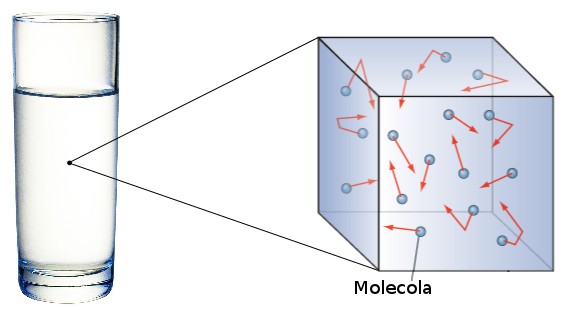
\includegraphics[scale=0.5]{Immagini/PuntoMacro.png}
\caption[Punto Macroscopico]{Punto Macroscopico}\label{fig: PuntoMacro}
\end{figure}

Un punto macroscopico di materiale continuo può essere modellizzato come una scatola cubica, di lato $L$ di estensione molto minore della dimensione lineare caratteristica del corpo, al cui interno sono contenute un numero $N$ (grande paragonabile al numero di Avogadro) di particelle, le molecole fondamentali costituenti l'oggetto.
In questo articolo si intendono studiare la dinamica molecolare classica, pertanto le particelle microscopiche verranno modellizzate come semplici punti materiali (\emph{Punti Microscopici}) sottostanti alle leggi della dinamica di Newton.

La scommessa della dinamica Molecolare è quella di dedurre lo stato macroscopico di un punto di un corpo continuo risolvendo la dinamica di un sistema microscopico opportunamente modellizzato.
La teoria fisica sottostante è molto semplice, il punto macroscopico è semplicemente un sistema classico  a molte particelle, la complicazione viene portata dal grande numero di sistemi elementari che vanno studiati contemporaneamente, in questo caso l'aiuto del calcolo computazionale diventa indispensabile. 

In conclusione il cuore di qualsiasi modello di Dinamica Molecolare classica saranno gli algoritmi di simulazione dei sistemi a molte particelle.

\subsection{Dinamica dei sistemi a Molte Particelle}\label{cap: Intro dinamica}
I sistemi che verranno considerati saranno una collezione di $N$ punti materiali di massa $m$ in uno spazio $\mathbb{R}^d$.
La cinematica del sistema verrà specificata fornendo la descrizione dei vettori
\begin{displaymath}
\vec{\mathbf{R}}=(\vec{r_1},\ldots,\vec{r_N}) \qquad \vec{\mathbf{V}}=(\vec{v_1},\ldots,\vec{v_N}) \qquad \vec{\mathbf{A}}=(\vec{a_1},\ldots,\vec{a_N}) 
\end{displaymath}
in funzione del tempo.

Ci si limiterà a considerare il sistema come isolato, le uniche interazioni saranno quelle esercitate reciprocamente dalle particelle costituenti. Le Forze verranno assunte conservative, la forma del potenziale corrispondende verrà considerata additiva e a due corpi (le interazioni a molti corpi verranno trascurate) pertanto l'equazione dell'energia interna del sistema assumerà la forma:
\begin{displaymath}
\mathcal{U}(\vec{\mathbf{R}}) = \sum\sum_{i>j}u(r_{ij})
\end{displaymath}
dove $u(r_{ij})$ è il potenziale di interazione tra due particelle poste a distanza scalare $r_ij = |\vec{r_i}-\vec{r_j}|$.


Come detto in precedenza la dinamica è classica, quindi la traiettoria di ogni particella dovrà soddisfare l'equazione di Newton:
\begin{displaymath}
\vec{F}_i = - \dfrac{\textrm{d}}{\textrm{d}\vec{r_i}} \Bigr(\sum_{j \neq i}u(r_{ij}) \Bigr) = m \cdot \vec{a_i}
\end{displaymath}
nel complesso l'evoluzione risulterà regolata da un sistema di $N$ equazioni differenziali di questo tipo.

In un sistema isolato l'energia meccanica totale $ E = K + \mathcal{U} $ dovrà essere costantemente conservata. Inoltre ponendosi nel sistema di riferimento del centro di massa la forza totale $\vec{\mathbf{F}}$ e il momento totale $\vec{\mathbf{P}}$ dovranno risultare costantemente nulli.
\medskip\newline
Ciò che veramente interesserà determinare del sistema microscopico saranno le sue osservabili collettive che definiscono lo stato termodinamico del sistema nel suo complesso (si contrappongono alle variabili $(\vec{\mathbf{R}},\vec{\mathbf{V}}$ che invece fissano lo stato microscopico del sistema). \newline
Per un sistema di $N$ particelle contenute in volume $V=L^d$ si definiscono:

\begin{itemize}
\item \underline{Temperatura} $T$. Per il teorema di equipartizione dell'enegia risulta l'equazione:
\begin{equation}\label{eq: temperatura}
K = \dfrac{d}{2}N k T
\end{equation}
che definisce la temperatura istantanea della configurazione, il suo valore osservabile sarà una media temporale su molte configurazioni.

\item \underline{Pressione} $P$. Dal teorema del viriale risulta l'equazione:
\begin{equation}\label{eq: Pressione}
Z = \dfrac{P V}{N kT} = 1 + \dfrac{1}{d N kT} \Biggr\langle \sum_{i=1}^N \vec{r_i}\cdot\vec{F_i}\Biggr\rangle
\end{equation}
dove $Z$ viene chiamato \emph{Fattore di comprimibilità} e con $\langle \cdot \rangle$ si intende la media temporale su molte configurazioni.

\item \underline{Densità} $\rho$. Definita come il rapporto tra la massa totale delle particelle e il volume che le contiene. In un sistema classico non sono previsti fenomeni di creazioni o deformazione dei gradi di libertà interni delle particelle, pertanto sarà una costante a meno di scambi di materia del sistema con l'ambiente circostante.
\end{itemize}
Se il sistema si trova in uno stato di equilibrio termodinamico queste osservabili saranno delle costanti dell'evoluzione temporale del sistema.

\medskip
Ciò che distinguerà un modello di meccanica molecolare classica da un altro sarà la definizione della forma specifica del potenziale $u(r_{ij})$ di interazione a due corpi. Si riconoscono due classi di sistemi: quello dei corpi soffici, per cui le forze intermolecolari sono funzioni continue della distanza tra le molecole, e quella dei corpi duri dotati di potenziali discontinui.





\FloatBarrier
\subsection{Simulazione Computazionale dei sistemi a Molte Particelle}\label{cap: Simulazione in Generale}
Tutti gli algoritmi di simulazione di dinamica molecolare classica presentano degli aspetti comuni.

\begin{itemize}
\item \underline{Numero di Particelle e Limite Termodinamico}\newline
Se ci si aspetta che questi modelli descrivano il comportamento di una piccola porzione di un corpo continuo bisognerà considerare un numero di molecole paragonabile al numero di Avogadro ($N_A = 6,022 \cdot 10^23$), una quantità di variabili troppo grande per essere trattata in modo efficiente da un computer.

In una simulazione computazionale si è obbligati a considerare un numero molto minore di particelle da quelle richieste teoricamente, questo limite determina degli errori sistematici sui valori ottenuti rispetto al valore atteso degli osservabili nel punto del sistema macroscopico.

Questo vincolo di $N\ll N_A$ imposto dai limiti tecnici della simulazione non si può eliminare direttamente ma si può aggirare, ottenendo comunque una buona stima del valore d'aspattazione teorico, tramite un'estrapolazione dei dati.
\newline
Calcolando il valore d'aspettazione di un osservabile per numerosi sistemi nelle stesse condizioni termodinamiche (densità e temperatura) ma con numero di particelle diverso (sufficientemente grande da evitare situazioni patologiche per i potenziali ma limitato in modo da mantenere contenuto il tempo macchina necessario all'esecuzione) ed eseguendo un fit di tali dati in funzione di $N$ si potrà ottenere il valore atteso come il limite per $N\gg 1$ dell'andamento ottenuto (limite termodinamico).


\item \underline{Disposizione Iniziale delle particelle}\newline
Se lo scopo della simulazione del sistema a molte particelle è quello di simulare gli atomi costituenti un corpo macroscopico bisognerà come minimo imporre che la forma del potenziale sia repulsiva a corta distanza, ovvero che
\begin{displaymath}
u(r) \xrightarrow[r \rightarrow 0]{} \infty
\end{displaymath}
in modo da evitare che tutte le molecole collassiono in un solo punto.

Un potenziale di questo tipo non permette di inizializzare il sistema con posizioni casuali, questa disposizione determinerebbe con frequenza stati in cui alcuni atomi sono molto vicini gli uni agli altri dando vita ad interazioni repulsive eccessivamente intense che distorcerebbero la dinamica del sistema.

La soluzione migliore per controllare questo problema è di disporre le posizioni iniziali delle particelle del sistema lungo un reticolo ordinato (solitamente \emph{Cubico a Corpo Centrato} o BCC), dopo un certo lasso di tempo detto \emph{termalizzazione}, l'azione continua delle interazioni porterà il sistema ad evolversi verso una configurazione più probabile.
	\begin{figure}[h!]
		\centering
		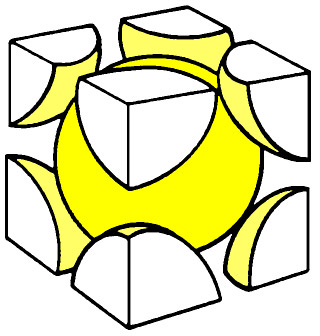
\includegraphics[scale=0.45]{Immagini/BCC.jpg}
		\caption[BCC]{Disposizione in reticolo BCC}\label{fig: BCC}
	\end{figure}


\item \underline{Inizializzazione delle velocità}\newline
Ciò che interessa studiare è un punto del continuo macroscopico a riposo, quindi è naturale porsi in un sistema di riferimento solidale con il centro di massa delle $N$ particelle microscopiche.
In questo caso il momento totale del sistema dovrà essere necessariamente nullo.

Per ottenere questa condizione è sufficiente inizializzare le componenti delle velocità di tutte le particelle in modo casuale , con $-1 < \vec{V}\cdot\hat{n} < 1$ ($\hat{n}$ versore di un asse del sistema cartesiano della "scatola"),e in seguito riscalare tutte le velocità in modo che il momento totale risulti azzerato:
\begin{displaymath}
\vec{v_i} \longmapsto \vec{v_i}\cdot \dfrac{1}{\sum_{i}^{}\vec{v_i}}
\end{displaymath}


\item \underline{Condizione di Bordo Periodico}\newline
Per rappresentare un punto di un porzione continua di materiale il sistema non può essere considerato una scatola immersa nel vuoto ma deve essere necessariamente circondato da sistemi dello stesso tipo posti a distanza trascurabile rispetto alla dimensione caratteristica del blocco di sostanza. 
Il sistema va quindi considerato confinato in una scatola cubica con altre scatole cubiche dello stesso tipo adiacenti ad ogni faccia, queste scatole modellizzano un insieme di punti macroscopici del materiale infinitamente vicini tra loro. 

Solitamente lo studio è finalizzato a studiare un punto in equilibrio termodinamico con il resto di materiale a lui vicino, quindi tutti gli altri sistemi adiacenti dovranno trovarsi in uno stato microscopico simile al sistema considerato.
\newline
Questa condizione viene approssimata considerando tutti i sistemi adiacenti, in ogni direzione, nello stesso identico stato microscopico del sistema preso in esame. 

	\begin{figure}[htbp]
		\centering
		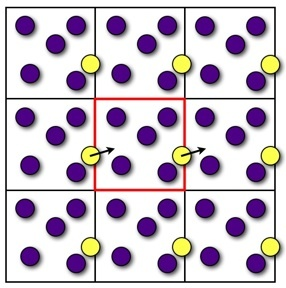
\includegraphics[scale=0.5]{Immagini/BordoPeriodo.jpg}
		\caption[Bordo Periodico]{Bordo Periodico e metodo delle immagini.}\label{fig: BordoPeriodo}
	\end{figure}

Pertanto quando si computeranno le interazioni esercitate su una particelle non si potranno considerare solo le interazioni con le altre particelle del sistema contenute nella scatola ma anche quella con tutte le altre nei sistemi limitrofi che saranno copie esatte delle particelle del sistema traslate di un unità di lato $L$.
(Quando si considerà questa approssimazione sarà necessario provvedere a "tagliare" la forma della funzione potenziale in modo da poter considerare nulla l'interazione ad una certa distanza).

Resta da considerare che a queste condizioni la scatola contenente il sistema non può essere assunta infinita, infatti può capitare che una particella esca dalla scatola e entri nel volume adiacente.

La \underline{condizione di bordo periodico} è la soluzione ideale per tenere conto di questo scabio termodinamico tra sistemi identici, un bordo di questo tipo compensa l'uscita della particella da una parete dellla scatola con l'ingresso di una particella identica dalla faccia opposta della scatola.


\item \underline{Termalizzazione}\newline
All'inizializzazione la distribuzione delle componenti delle velocità sarà uniforme, ovvero i campioni delle velocità del sistema saranno egualmente distribuite in un intervallo prestabilito.
Lasciando evolvere naturalmente il sistema iniziale ordinato (in un reticolo BCC) per un intervallo di tempo sufficientemente grande il sistema si troverà in una configurazione ormai indipendente da quella inziale e soddiferà le ipotesi della distribuzione di \emph{Maxwell-Boltzman}.
In questo caso l'insieme di una determinata componente cartesiana delle velocità di tutte le particelle costituenti il sistema soddisferà una distribuzione gaussiana di questo tipo:
\begin{equation}
f(v_i) dv_i = \dfrac{1}{N} \: N(v_i) dv_i = \dfrac{1}{\mathcal{N}} \: e^{-A v_i^2} \qquad 
\textrm{dove} \; \mathcal{N} = \sqrt{\dfrac{\pi}{A}} \;\; \textrm{e} \;\; A = \dfrac{1}{2}\dfrac{m}{kT}
\end{equation}
qualsiasi sia la componente $i$ considerata.

In un sistema con un numero $N$, finito e piccolo, di particelle non è possibile stimare una distribuzione continua. In tal caso lo studio dell'istogramma normalizzato dei valori delle velocità è un buon criterio per determinare la corretta termalizzazione del sistema simulato. 
Per raffinare un grafico di questo tipo , oltre ad aumentare il numero di particelle della simulazione, si può incrementare la statistica raccolta accumulando velocità per diversi configurazioni a tempi successivi, se il sistema è effettivamente termalizzato i dati saranno compatibili e il sistema oscillerà tra configurazioni di equilibrio equiprobabili.

In alternativa si può valutare la funzione di Boltzman che associa ad ogni configurazione un valore definito da:
\begin{equation}
H_x = \int dv_x f(v_x) \ln{\biggr(f(v_x)\biggr)} = \sum_{\Delta v_x}^{}f(v_x) \ln{ \biggr(f(v_x)\biggr)} \Delta v_x
\end{equation} %=  - \dfrac{1 + \ln{(\mathcal{N}})}{2}
dove nell'ultima eguaglianza è data la versione per un sistema finito tramite integrazione per rettangoli dell'istogramma.
Quando la distribuzione presenta l'andamento gaussiano previsto risulterà:
\begin{equation}
H_i = \dfrac{1}{\mathcal{N}}\int dv_x \, e^{-A v_i^2} \, \ln{(\dfrac{e^{-A v_i^2}}{\mathcal{N}})} 
= \dfrac{-1}{\mathcal{N}} \Biggr( \int dv_x(A\, v_i^2)\, e^{-A v_i^2} + \ln{\mathcal{N}}\int dv_x e^{-A v_i^2}  \Biggr)
=- ( \dfrac{1}{2} + \ln{\mathcal{N}})
\end{equation}

Il discorso sull'aumento della statistica raccolta si applica anche in questo caso visto che l'integrale è calcolato sulla disribuzione discretizzata (l'istogramma).

[h!]
\item \underline{Grandezze Adimensionate}\newline
Il calcolatore può trattare solo numeri puri quindi prima di implementare una qualsiasi algoritmo computazionale è necessario stabilire delle unità dimensionali specifiche del sistema in modo da poter interpretare fisicamente i dati ottenuti dalla simulazione.
Un procedimento sicuro per ottenere un sistema di unità di misura classico completo è fissare tre unità tra MASSA LUNGHEZZA ENERGIA E TEMPO in modo da poter esprimere ogni altra grandezza derivata in funzione di esse.
La scelta verrà effettuata sfruttando i parametri dimensionali caratteristici di ogni specifica simulazione.


\item \underline{Studio delle Transizioni di Fase}\newline
Come già detto lo scopo di questo studio è di derivare il comportamento fisico macroscopico dei continui come manifestazione della struttura microscopica della materia.
Per un campione di materiale macroscopico si riconoscono almeno 3 stati fisici di aggregazione solido, liquido  e gassoso.
Ci si aspetta che una simulazione di dinamica molecolare ben definita possa simulare, a seguito di una corretta termalizzazione, almeno una transizione da solido a  fluido al variare delle variabili di stato( pressione, volume e temperatura).

Per semplicità si studia l'andamento di P in funzione di $\rho$ e T che sono variabili più facili da fissare durante l'inizializzazione del sistema, in tal caso si dice che la Pressione funge da parametro d'ordine.
Ci si aspetta quindi che una qualsiasi irregolarità o discontinuità dell'andamento del parametro d'ordine, incompatibile con gli errori statistici sulla misura, possa essere sintomo di una transizione di fase del sistema.

Oltre al parametro d'ordine $P$ è possibile studiare la diffussione per rilevare la fase in cui si trova il sistema.
La differenza principale che intercorre tra un sistema in fase solida e in fase fluida e la libertà di movimento delle molecole.
In un sistema solido  le particelle sono vincolate ad occupare una posizione prefisata in un reticolo potendo al limite oscillare attorno ad una posizione d'equilibrio.
Al contrario in un sistema liquido o gassoso le particelle sono libere di fluire nel volume, attraversarlo e in sufficiente tempo anche uscire da esso.

\begin{figure}[h!]\vspace{-5pt}
     \begin{minipage}{0.55\textwidth}
		\begin{flushright}
		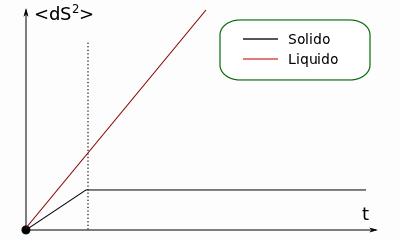
\includegraphics[scale=0.5]{Immagini/dS_quad_exp.png}
		\end{flushright}
     \end{minipage}\hfill
     \begin{minipage}{0.4\textwidth}
     	\begin{flushleft}
		\caption[Spostamento quadratico medio atteso]{Andamento atteso dello spostamento quadratico medio in funzione del tempo di diffusione.}\label{fig: dS_quad_exp}
     \end{flushleft}
     \end{minipage}\vspace{-5pt}
  \end{figure}

Per determinare il comportamento di diffusione caratteristico dello stato del sistema è utile misurare due osservabili.
La prima è lo \emph{spostamento quadratico medio} delle particelle :
\begin{equation}
\biggr\langle dS^2(t) \biggr\rangle = \biggr\langle\big\vert \vec{r_i}(t) - \vec{r_i}(0) \big\vert^2  \biggr\rangle
\end{equation}
dove la distanza è misurata senza applicare la condizione di bordo, seguendo quindi le particelle non loro moto libero di diffusione eventualmente anche fuori dal volume iniziale, mentre la media e calcolata su numerose coppie di configurazioni a distanza temporale $t$ e su tutte le particelle.

L'andamento atteso è mostrato nella figura \ref{fig: dS_quad_exp}, nella fase liquida le particelle propagheranno quasi linearmente diffondendo fuori dal volume, nella fase solida invece lo spostamente medio non potrà aumentare oltre il valore dell'oscillazione massima.
\medskip

La seconda quantità che si può studiare è la \emph{funzione di distribuzione radiale} $g_t(r)$, ovvero la distribuzione dei valori dello distanza, calcolato con la condizione di bordo periodico, tra la posizione occupata da una particella al tempo $t_0=0$ e la posizione in cui si trova la stessa particella dopo un evoluzione temporale di $t$ del sistema. Ovvero, per un sistema finito, corrisponde all'istogramma dei valori di:
\begin{equation}
dS(t) = \big\vert \vec{r_i}(t) - \vec{r_i}(0) \big\vert
\end{equation}
campionati per diverse coppie di configurazioni a distanza temporale $t$ e per tutte le particelle.
\newline
Per un sistema solido si attende che la distribuzione $g_t(r)$ risulti molto piccata intorno ad un valore $r_o\ll D_{max}$(modulo dell'ampiezza di oscillazione) dove con $D_{max}$ si intende la massima distanza che si può estendere tra 2 punti in un sistema quadrato con condizioni di bordo periodico:
\begin{equation}
D_{max}= \frac{\sqrt{d}}{2}
\end{equation}
Mentre per un sistema fluido, se il tempo di evoluzione $t$ è sufficientemente alto, ci si aspetta che la distribuzione di probabilità di trovare la particella in punto specifico della scatola sia uniforme ovunque, ovvero dopo l'evoluzione la particella potrà trovarsi in ogni altro punto del volume in modo completamente casuale.

\begin{figure}[htbp]
     \begin{minipage}{0.4\textwidth}
		\begin{flushright}
		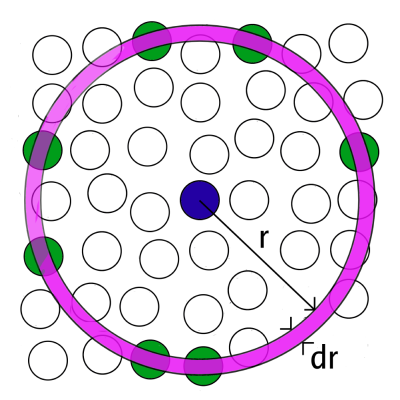
\includegraphics[scale=1.25]{Immagini/RDF.png}
		\end{flushright}
     \end{minipage}\hfill
     \begin{minipage}{0.55\textwidth}
     	\begin{flushleft}
		\caption[Funzione di Distribuzione Radiale]{\footnotesize Corona circolare che rappresenta l'elemento di superficie radiale a distanza $r$ dall'origine. Quando $r>L/2$ l'elemento non è più completamente inscritto nella scatola.}\label{fig: RDF}
     \end{flushleft}
     \end{minipage}
  \end{figure}

In tal caso la distribuzione radiale crescerà in accordo con la crescita del volumetto elementare (figura \ref{fig: RDF}). Più precisamente se $\mathcal{\tilde{\rho}}(P)=\textrm{cost}$ è la distribuzione di probabilità (uniforme) di trovare la particella nel punto $P$ dopo l'evoluzione temporale, risulterà che:
\begin{eqnarray}
g_t(r) dr &=& \mathcal{\tilde{\rho}} \cdot 2\pi r\,dr   \qquad \textrm{(in 2 dimensioni)}    \nonumber \\
g_t(r) dr &=& \mathcal{\tilde{\rho}} \cdot \pi r^2\,dr   \qquad \textrm{(in 3 dimensioni)}    
\end{eqnarray}
almeno per distanze minori di $L/2$. 
Per distanze maggiori invece l'elemento di volume tenderà a decrescere con l'aumentare della distanza, questo perchè sfere di raggio $L/2<r<D_{max}$ non possono essere completamente inscritte in un cubo di lato $L$, pertanto la distribuzione di probabilità tenderà a smorzarsi fino ad annullarsi a distanza $D_{max}$.
\begin{figure}[h!]\vspace{-10pt}
     \begin{minipage}{0.6\textwidth}
		\begin{flushright}
		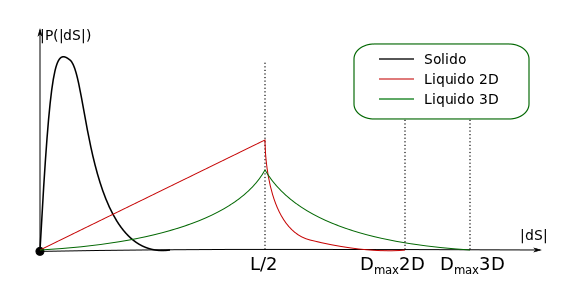
\includegraphics[scale=0.45]{Immagini/DistrodS.png}
		\end{flushright}
     \end{minipage}\hfill
     \begin{minipage}{0.4\textwidth}
     	\begin{flushleft}
			\caption[Distribuzione Radiale Attesa]{Andamento atteso delle distribuzioni radiali $g_t(r)$ a seconda della fase del sistema.}\label{fig: DistrodS}
     \end{flushleft}
     \end{minipage}\vspace{-15pt}
  \end{figure}
  
In conclusione risulterà un'andamento simile a quello mostrato nella figura (\ref{fig: DistrodS}).
% http://isaacs.sourceforge.net/phys/rdfs.html


\item \underline{Fasi Metastabili}\newline
In generale i sistemi considerati non mostrano delle transizioni di fase nette, presentano invece delle \emph{Fasi metastabili} intorno ad alcuni valori caratteristici delle variabili di stato.
In sistuazioni di questo tipo si osserva un'oscillazione caotica  del parametro d'ordine tra le curve caratteristiche della fase precedente e di quella successiva.
Infatti quando il sistema si trova in uno stato metastabile ha la possibilità di poter assumere caratteristiche di entrambe le fasi, non perchè si trova in una "via di mezzo" tra la fase liquida e la fase fluida ma perchè può termalizzare in una qualsiasi delle due a seconda di quali siano le condizioni iniziali scelte.
Quando il sisteam si trova in una condizione di questo tipo anche una piccola variazione dei parametri di stato può determinarare un netto cambiamento di fase, mostrando un comportamento simile al caos deterministico della "mappa logistica".

\end{itemize}
Nei prossimi capitoli verrano applicate concretamente queste linee guida per studiare 2 modelli specifici di dinamica molecolare: il modello \emph{a "sfere dure"} e il modello \emph{a "sfere soffici"} con potenziale di \emph{ Lennard-Jones}.

\clearpage
%/\/\/\/\/\/\/\/\/\/\/\/\/\/\/\/\/\/\/\/\/\/\/\/\/\/\/\/\/\/\/\/\/\/\/\/\/\/\/\/\/\/\/\
\section{Sfere Dure}\label{Dure}
In un modello di Dinamica Molecolare a sfere dure la forza di interazione intermolecolare è caratterizzata da una funzione discontinua della distanza corrispondente al potenziale:
\begin{equation}
u(r) =	\begin{cases} 
			\infty  & \mbox{se }r\leq \sigma \\
			0 		& \mbox{se }r> \sigma
		\end{cases}
\end{equation}
dove $\sigma$ è il diametro della particella.
In questo modello le particelle sono equivalenti a delle sfere completamente impenetrabili di diametro $\sigma$, l'unica interazione che si esercita tra loro è tramite collisioni totalmente elastiche.
\medskip \newline 
In un sistema di questo tipo non è necessario risolvere le equazioni differenziali del moto, le particelle si muovono di moto rettilineo uniforme ($a_i(t) = 0$) finchè non urtano con un'altra molecola.

Lo studio della cinematica si riduce ad un calcolo puramente algebrico basto su poche leggi fondamentali. Per ogni coppia di particelle $P_1$ e $P_2$, siano :
\begin{displaymath}
\vec{r}_{12} = \vec{r}_1 - \vec{r}_2 \qquad \vec{v}_{12} = \vec{v}_1 - \vec{v}_2
\end{displaymath}
i vettori di "separazione", vale che:

\begin{enumerate}
\item Le due particelle  collidono se e solo se:
\begin{equation}\begin{cases}\label{eq: condizioneurto}
 & \vec{v}_{12}\cdot \vec{r}_{12} < 0\\
 & \Delta = (\vec{v}_{12}\cdot \vec{r}_{12})^2 - v_{12}^2(r_{12}^2 -\sigma^2) \geq 0
\end{cases}\end{equation}
La prima condizione assicura che le due particelle siano in avvicinamento lungo la congiungente e la seconda assicura che ,ponendosi nel sistema di riferimento di una particella, la traiettoria dell'altra particella avrà una distanza di avvicinamento massimo minore di $\sigma$. 

\item Siano $\vec{r_1}$ e $\vec{r_2}$ i vettori posizione della coppia di molecole al tempo $t_0$, se le particelle soddisfano la condizione (1) urteranno al tempo:
\begin{equation}\label{eq: tempocollisione}
 t_c = t_0 + \dfrac{-(\vec{v}_{12}\cdot \vec{r}_{12}) - \sqrt{\Delta} }{v_{12}^2}
\end{equation}


\item Dopo la collisione le particelle urtanti variano la loro velocità secondo l'equazione:
\begin{equation}\begin{cases}\label{eq: cambiovel}
 \vec{v}_{1}' & = \vec{v}_{1} - \big[ (\vec{v}_{1} - \vec{v}_{2})\cdot \hat{r}_{12} \big] \hat{r}_{12}\\
 \vec{v}_{2}' & = \vec{v}_{1} + \big[ (\vec{v}_{1} - \vec{v}_{2})\cdot \hat{r}_{12} \big] \hat{r}_{12}
\end{cases}\end{equation}
 
 
\item Prima e dopo la collisione le particelle seguono una traiettoria rettilinea uniforme:
\begin{equation}
\vec{r}_i(t) = \vec{r}_i(t_0) + \vec{v}_i(t - t_0) \qquad \textrm{se } t<t_c
\end{equation} 
\end{enumerate}
Tali equazioni derivano direttamente dalla condizione di urto totalmente elastico, caratterizzato dalla conservazione di energia cinetica e di momento totale durante la collisione.


\subsection{Metodi Numerici e Simulazione Computazionale}
Prima di poter studiare numericamente la dinamica è necessario stabilire quali sono le costanti dimensionali che forniranno le unità di misura fondamentali per il studio del sistema.

\paragraph{Unità di Misura del sistema}
\begin{itemize}
\item[-] \underline{Massa}: $[M]=m=1$ 
\newline Tutte le particelle sono identiche e la loro massa fornisce l'unità di misura più ovvia.

\item[-] \underline{Lunghezza}: $[L]=L=1$ 
\newline Il diametro $\sigma$ costituirebbe un'altra scelta possibile, ma in questo caso risulta più comodo esprimerlo in unità di lato.

\item[-] \underline{Energia}: $[E]=kT=1$ 
\newline L'energia totale del sistema è conservata e puramente cinetica, per il principio di equipartizione (eq: \ref{eq: temperatura}) è proporzionale alla temperatura del sistema. 
\end{itemize}

Scegliere la temperatura come unità significa che verranno simulati sempre sistemi con $kT=1$, gli osservabili calcolati per sistemi a temperatura diversa si otterranno dal primo tramite un semplice fattore di cambio di unità di misura. Il discorso vale in modo analogo anche per le distanze e le masse.
Ad esempio, se per un sistema unitario si misura un tempo di collisione pari a $t^{*}$, per il generico sistema corrisponderà un valore:
\begin{displaymath}
t_c= t^* \biggr[L\sqrt{\dfrac{m}{kT}} \biggr]
\end{displaymath}
\newline\medskip

\FloatBarrier
\subsubsection{Algoritmo di Evoluzione del sitema: Metodo della tavola delle collisioni}
L'evoluzione del sistema è determinata dalle collisioni, per tenere conto di quali particelle urtano per prime si costruisce una tabella detta \emph{tavola delle collisioni} che all'ingresso $(i,j)$ contiene il tempo che impiegherebbero le particelle $P_i$ e $P_j$ a collidere fra di loro in assenza di altri ostacoli.
Questi tempi $Tc_{i,j}$ vengono calcolati considerando anche la condizione di bordo periodico, per cui le particelle possono urtare tra di loro anche dopo aver attraversato il bordo della scatola ed essere rientrare dalla parete opposta.
\medskip\newline
Per tenere conto di questa possibilità si usa il metodo delle \emph{Particelle Immagine} per cui il tempo di collisione tra le particelle $P_i$ e $P_j$ viene calcolato come il minimo fra i tempi di collisione della particella $P_i$ con tutte le copie di $P_j$ che si trovano nei sistemi identici limitrofi al volume del sistema considerato (ovviamente il minimo viene calcolato considerando anche la particelle originaria all'interno della scatola).
\medskip\newline
Chiaramente due particelle non devono collidere necessarimente con le copie più vicine, potrebbero collidere più lontano o non collidere affatto. Questo non determina un problema se si ha l'accorgimento di inizializzare il sistema con una densità di particelle sufficientemene alta. In tal caso, anche se una coppia non collide, avverranno altre collisioni che permettono al sistema di rimerscolarsi. 
In questo caso non sarà necessario calcolare i tempi di collisione con le copie immagini molto distanti, basteranno solo le copie più vicine in modo da tenere correttamente conto di tutte le collisioni che avvengono in prossimità dei bordi del sistema e che altrimenti verrebbero ignorate.
\medskip\newline
La tavola delle collisioni viene costruita una sola volta in fase iniziale, dopo di che il sistema evolverà, un urto alla volta, secondo il seguente algoritmo:

\begin{tikzpicture}[node distance = auto]
    % Place nodes
    \node [block_largo] (1) {Determinazione della prossima coppia di particelle urtanti e il loro tempo di Collisione. \newline \footnotesize( Trovare le coordinate $i,j$ corrispondenti all minimo della tavola delle collisioni e il suo valore $t_c$)};
    \node [block_largo, below of=1,node distance=2.25cm] (2) {Evoluzione del sistema fino al tempo di collisione. \newline \footnotesize( Evolvere le posizioni di tutte le particelle $\vec{r_i} \mapsto \vec{r_i} + \vec{v_i} \cdot t_c $)};
    \node [block_largo, below of=2,node distance=2.25cm] (3) {Applicazione della condizione di bordo periodico a tutte le particelle che sono uscite dal volume. \newline \footnotesize( Per ogni componente se $ r_x \geq L \Rightarrow r_x \mapsto r_x - L $ oppure se $ r_x<0 \Rightarrow r_x \mapsto r_x + L $ )};
    \node [block_largo, below of=3,node distance=2.25cm] (4) {Aggiornamento delle velocità delle particelle urtanti. \newline \footnotesize( Evolvere la posizione delle particelle urtanti $\vec{v_i} \mapsto \vec{v_i} - \vec{\Delta V}$ e $\vec{v_j} \mapsto \vec{v_j} + \vec{\Delta V}$ secondo la formula.)};
    \node [block_largo, below of=4,node distance=2.25cm] (5) {Aggiornamento della tavola di collisione. \newline \footnotesize( Si riscrivono solo la i-sima e j-sima colonna della tavola delle collisioni, ricalcolando i tempi di collisione relativi alle due particelle $i,j$ considerando la nuova velocità che hanno assunto dopo l'urto.)};


    % Draw edges
    \path [line] (1) -- (2);
    \path [line] (2) -- (3);
    \path [line] (3) -- (4);
    \path [line] (4) -- (5);
	\path [line] (5) -- +(9.5,0)  |- (1); 
 
\end{tikzpicture}

\FloatBarrier
\subsubsection{Implementazione computazionale dell'algoritmo}
Per simulare questo sistema verrà sfruttata la programmazione ad oggetti del linguaggio C++.
L'idea è di definire una classe \Cls{sistema\_rigido()} che contenga tra i suoi parametri tutti i dati necessari per definire lo stato microscopico del sistema, in questo caso gli attributi fondamentali saranno:
i definire la classe \Cls{sistema\_soffice()} dotata degli attributi necessari a descrivere lo stato microscopico del sistema:
\begin{itemize}
\item 2 array di vettori per memorizzare posizione e velocità di tutte le particelle costituenti il sistema.

\item 1 array bidimensionale per salvare la tavola delle collisioni.

\item 3 variabili \emph{double} per contenere le costanti $\sigma$, $L$, $\eta$ del sistema. 2 varibili \emph{int} per salvare il numero di particelle e la dimensione spaziale della simulazione.

\end{itemize}
%\medskip\newline
Il costruttore della classe costituirà la fase di \emph{inizializzazione} dell'algoritmo, ovvero salverà le posizioni inziali in bcc, fornirà velocità iniziali casuali riscalandole a Momento totale nullo e a temperatura unitaria e infine costruirà la tavola delle collisioni completa.
Le variabili richieste per inizializzare il sistema saranno la dimensione spaziale $d$, la funzione di impacchettamento $\eta = V_\textrm{particelle} / V_\textrm{scatola}$ e il numero $L$ di particelle disposte lungo una riga del reticolo iniziale.
\medskip\newline
Il metodo \cd{evoluzione()} sarà il cardine della simulazione, questa funzione fornisce l'evoluzione temporale del sistema dalla configurazione corrente fino al primo urto in accordo con l'algoritmo precedente.
\medskip\newline
La fase di \emph{termalizzazione} si otterrà applicando questo metodo un numero di volte sufficiente a realizzare la distribuzione di Maxwell-Boltzman per le velocità.
\medskip\newline
Similmente la fase di \emph{produzione} si realizza intervallando la raccolta di osservabili istantanei sulla configurazione del sistema all'evoluzione temporale necessaria per ottenere un'altra configurazione sufficientemente scorrelata dalla prima.
\medskip\newline
Per ottenere rapidamente una successione di sistemi inizializzati con un parametro $\eta$ differente si usa il metodo \cd{rinizializzazione()} che prende in ingresso un nuovo valore della frazione di impacchettamento (più piccolo del precedente) e si limita ad aggiornare il parametro $\sigma$ rimpicciolendo il raggio delle sfere ma conservando la disposizione e le velocità ottenute dalle simulazioni precedenti.

\FloatBarrier
\subsection{Caratteristiche dell'algoritmo di Simulazione}
Dall'osservazione della disposizione delle particelle del sistema dopo diversi urti si possono dedurre le prime considerazioni qualitative sulle proprietà del sistema.
Nella figura (\ref{fig: snap2d}) sono mostrate 4 istantanee delle configurazioni in cui si trova il sistema in seguito alla termalizzazione a vari valori di $\eta$.
Dall'immagine si nota come siano presenti due fasi distinte e come la transizione tra di esse sia di natura puramente geometrica. Essendo le molecole impenetrabili al superamento di un certo valore di densità non ci sarà più possibilità di diffusione, infatti tenderanno ad incastrarsi tra di loro  disponendosi in un reticolo (di forma esagonale con particella centrale) più "denso" della disposizione BCC scelta in partenza.
\begin{figure}[htbp]
		\caption[Sfere Rigide$/$Preliminari\_Snap2D.cpp]{Immagini del sistema 2D termalizzato a diversi valori di impacchettamento. (In alto a sinistra è visibile la configurazione inziale prima dell'evoluzione temporale).}	\vspace{-15pt}
        \begin{subfigure}[b]{0.5\textwidth}
                \centering
                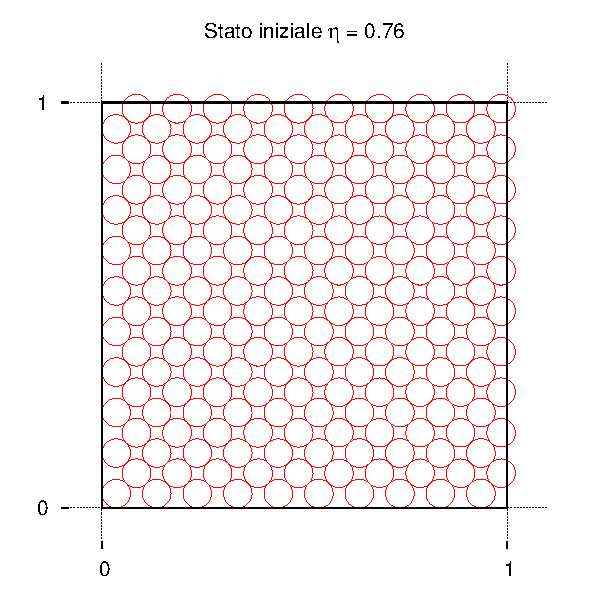
\includegraphics[width=0.85\textwidth]{Immagini/Rigide/SnapInizio_2D}
        \end{subfigure}%
        ~ %add desired spacing between images, e. g. ~, \quad, \qquad etc. 
          %(or a blank line to force the subfigure onto a new line)
        \begin{subfigure}[b]{0.5\textwidth}
                \centering
                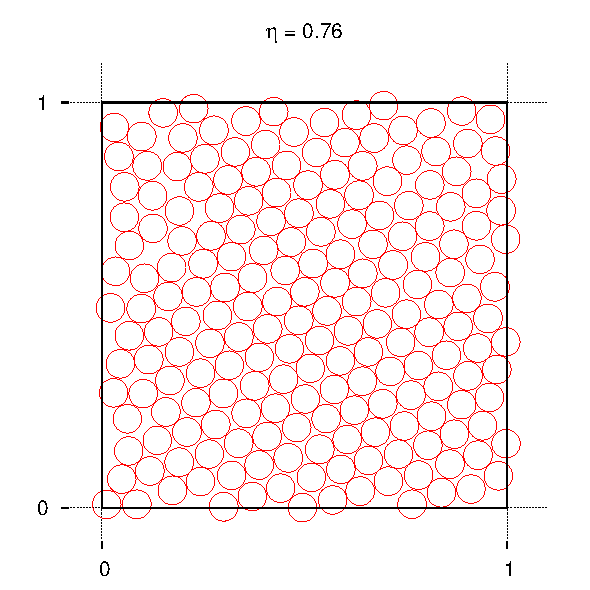
\includegraphics[width=0.85\textwidth]{Immagini/Rigide/SnapSolido_2D}
        \end{subfigure}
        ~ %add desired spacing between images, e. g. ~, \quad, \qquad etc. 
          %(or a blank line to force the subfigure onto a new line)
\vspace{-15pt}

        \begin{subfigure}[b]{0.5\textwidth}
                \centering
                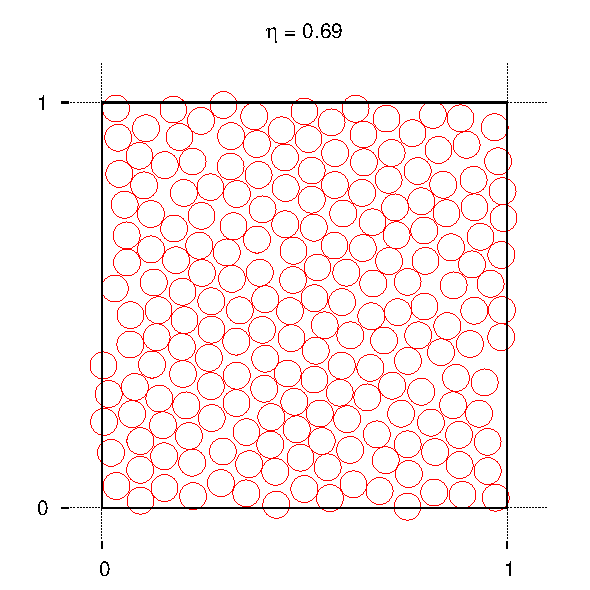
\includegraphics[width=0.85\textwidth]{Immagini/Rigide/SnapMeta_2D}
        \end{subfigure}
                \begin{subfigure}[b]{0.5\textwidth}
                \centering
                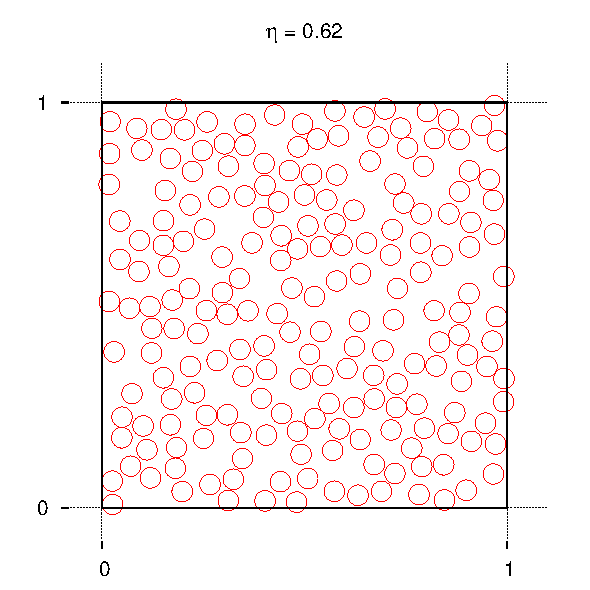
\includegraphics[width=0.85\textwidth]{Immagini/Rigide/SnapLiquido_2D}
        \end{subfigure}
		
		 \centering  \footnotesize{$N= 200$ , $d=2$ , N urti evoluzione=$ 200 $ per particella}
		\label{fig: snap2d}
\end{figure}

\subsubsection{Tempo di esecuzione}
La maggior parte dello sforzo computazionale viene ovviamente investita nel calcolo dei singoli step di evoluzione temporale.
Nella figura (\ref{fig: TempoEsecuzione}) è mostrato l'andamento del tempo di esecuzione medio necessario per il calcolo di una singola evoluzione in funzione del numero di particelle del modello.
\begin{figure}[htbp]
	\centering
\caption[Sfere Rigide$/$Preliminari\_TempoEsecuzione.cpp]{Andamento del tempo macchina medio necessario a calcolare un passo d'evoluzione in funzione del numero di particelle.}\vspace{-15pt}
	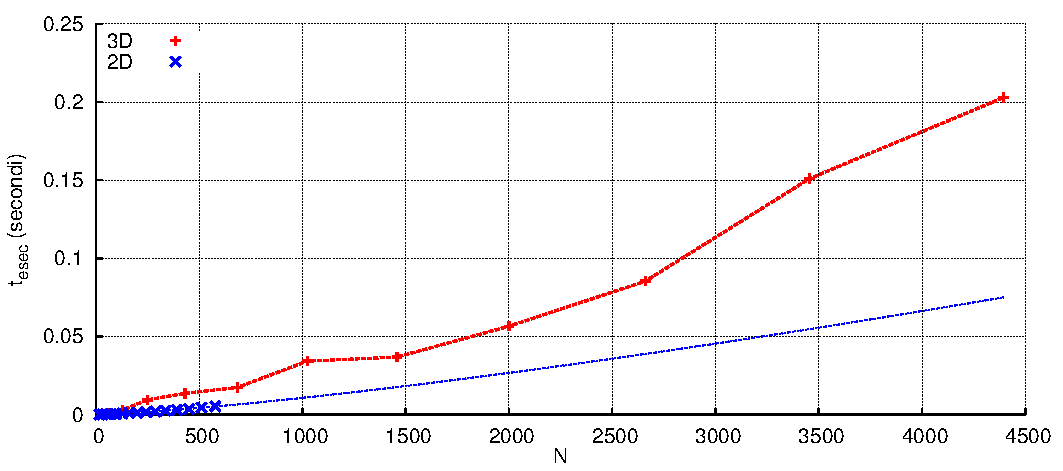
\includegraphics[scale=0.95]{Immagini/Rigide/T_esec}
	\newline \footnotesize{$\eta_{2D}= 0.7$ , $\eta_{3D}= 0.515$ , media su $10000$ collisioni}
	\label{fig: TempoEsecuzione}
\end{figure}
Naturalmente il tempo macchina necessario dipenderà dal numero di particelle, infatti il numero di coppie che possono essere coinvolte in una collisione risulta:
\begin{displaymath}
N_\textrm{coppie} = \dfrac{N (N-1)}{2}
\end{displaymath}
quindi il tempo necessario per ricalcolare la tavola di collisione e calcolarne il minimo aumenta di conseguenza.
\newline
Dal grafico è anche evidente la forte dipendenza dalla dimensione spaziale del modello. Questo dato entra pesantemente nel calcolo dei tempi di collisione con il metodo delle immagini, infatti il numero di copie che vanno considerate aumenta con la dimensione come $ N_\textrm{immagini} = 3^d $.


\subsubsection{Tempo di Termalizzazione}
Per poter effettuare una raccolta effettiva delle caratteristiche del modello in un determinato stato è necessario disporre di una configurazione correttamente termalizzata.
Per stabilire il numero di collisioni necessari a portare il sistema nella condizione prescelta si procede allo studio della funzione di Boltzman in funzione degli step evolutivi.

\begin{figure}[htbp]
\centering
	\caption[Sfere Rigide$/$Preliminari\_Termalizzazione.cpp]{Andamento della funzione di Boltzman istantanea e media in funzione del numero di passi evolutivi.}
	\vspace{-15pt}
	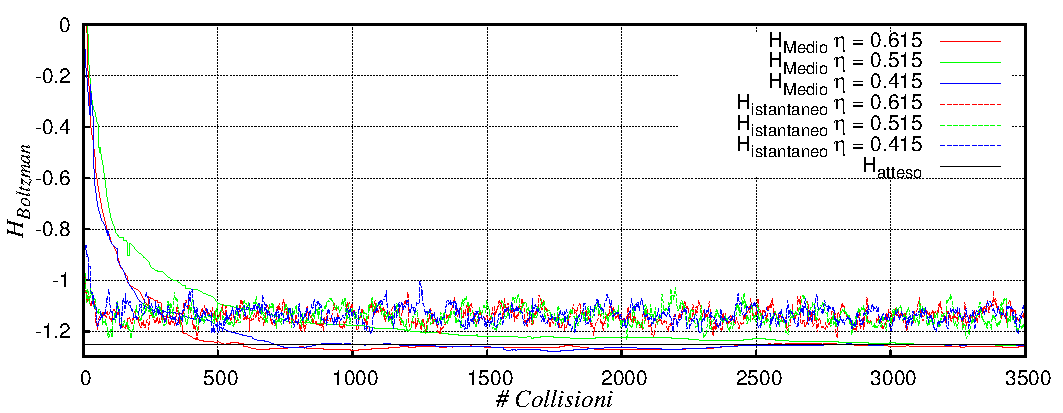
\includegraphics[scale=0.95]{Immagini/Rigide/HvsStep3D}
	\newline\footnotesize{$N= 686$ , $d=3$ , campioni raccolti ogni urto.}
	\label{fig: Termalizzazione}
\end{figure}

Dal grafico (\ref{fig: Termalizzazione}) si nota come l'andamento della funzione $H$ istantanea continui a rimanere piuttosto rumoroso durante l'evoluzione del sistema, questo effetto è dovuto al basso numero di particelle che con una sola configurazione campionata fornisce una statistica insufficiente allo studio della distribuzione di probabilità.
\newline
L'andamento della funzione mediata è invece più regolare. La convergenza al valore atteso avviene in media dopo 10 urti per particella lontano dalla fase metastabile che richiede più tempo per essere termalizzare rispetto agli altri valori di $\eta$.

\begin{figure}[htbp]
\centering
\caption[Sfere Rigide$/$Preliminari\_Termalizzazione.cpp]{Distribuzione delle componenti x delle velocità dopo N passi.}
	\vspace{-15pt}
	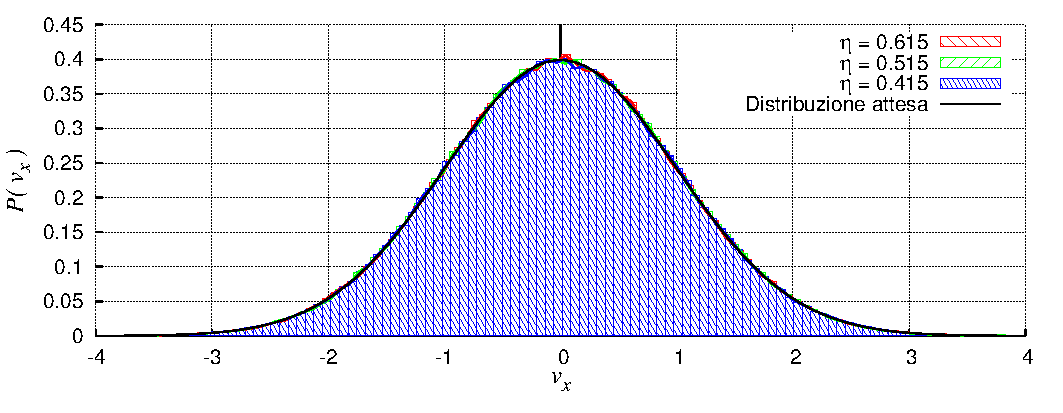
\includegraphics[scale=0.95]{Immagini/Rigide/DistroVx}
	\newline
	\footnotesize{$N= 686$ , $d=3$ , campioni$= 5000$ per particella, intervallo di raccolta campioni = $1$ urto per particella,  urti termal=$ 5000 \cdot N$.}
	\label{fig: IstoTermalizzazione}
\end{figure}

Nella figura (\ref{fig: IstoTermalizzazione}) si può osservare come in seguito della termalizzazione la distribuzione delle velocità sia la stessa per tutte le fasi e sia in accordo con la distribuzione gaussiana attesa.

\FloatBarrier
\subsection{Caratteristiche del modello, studio delle transizioni di fase}
Come era intuibile dalla figura (\ref{fig: snap2d}), il sistema a sfere rigide è in grado di presentare una transizione di fase nonostante sia dotato di un potenziale d'interazione molto semplice.
Si procede quindi allo studio di questo fenomeno come indicato nelle linee guida del capitolo \ref{cap: Simulazione in Generale}.
\subsubsection{Studio del fattore di comprimibilità come parametro d'ordine}
Nel capitolo precedente è stato introdotto il fattore di comprimibilità come media sui momenti angolari delle forze (equazione \ref{eq: Pressione}).
Le sfere dure, però, esercitano solo una forza di durata istantanea nel momento esatto in cui avviene la collisione. 
In questo caso è necessario dedurre un'espressione per $Z$ specifica per questo modello, sfruttando il teorema dell'impulso si ottiene:
\begin{equation}\label{eq: termPRigido}
Z = \dfrac{P V}{N kT} = 1 + \dfrac{m}{d N kT} \dfrac{1}{t} \sum_{c=1}^{N_c}\vert \Delta \vec{v}_{ij}(t_c) \vert 
\end{equation}
dove $t$ è il tempo trascorso durante le $N_c$ collisioni e $\Delta \vec{v}_{ij}(t_c)$ è il vettore che da la variazione di velocità subita dalla coppia di particelle urtante nell'istante $t_c$.

\begin{figure}[htbp]
\centering
\caption[Sfere Rigide$/$PvsEta\_2D.cpp]{Andamento dal parametro d'ordine $Z$ in funzione della frazione d'impacchettamento.}	\vspace{-15pt}
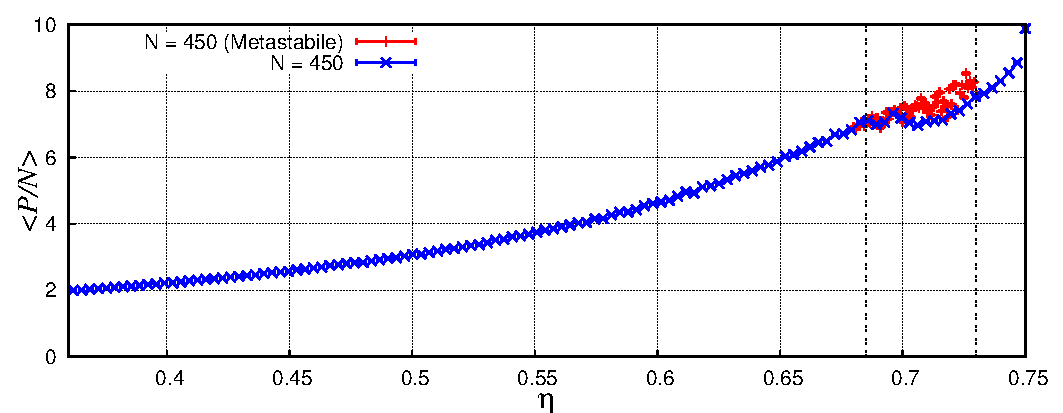
\includegraphics[scale=0.9]{Immagini/Rigide/PvsEta2D}
	\newline \footnotesize{$N= 450$ , $d=2$ , campioni$= 100$ per particella,  urti termal=$ 50 \cdot N$}
	\label{fig: PvsEta2D}
\end{figure}

\begin{figure}[htbp]
\centering
\caption[Sfere Rigide$/$PvsEta\_3D.cpp]{Andamento dal parametro d'ordine $Z$ in funzione della frazione d'impacchettamento.}	\vspace{-15pt}
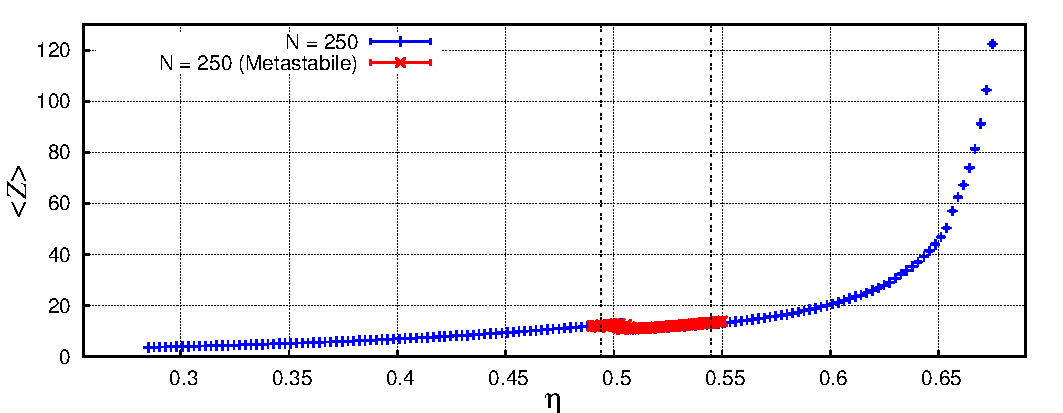
\includegraphics[scale=0.9]{Immagini/Rigide/PvsEta3D}
	\newline \footnotesize{$N= 250$ , $d=3$ , campioni$= 100000$ ,  urti termal=$ 50 \cdot N$}
	\label{fig: PvsEta3D}
\end{figure}
Nelle figure (\ref{fig: PvsEta2D}) e (\ref{fig: PvsEta3D}) è mostrato l'andamento del parametro d'ordine $Z$ in funzione della frazione d'impacchettamento $\eta$.
Dai grafici si stima la presenza di una fase metastabile nei seguenti intervalli:

\begin{center}
\begin{tabular}{|c|r c l |}
\hline
	$2D$ & 0.685 & $<\eta_{\textrm{meta}}<$ & 0.735 \\
\hline
	$3D$ & 0.49 & $<\eta_{\textrm{meta}}<$ & 0.55\\
\hline
\end{tabular}
\end{center}
La natura instabile del sistema in queste regioni può essere evidenziata da un secondo calcolo del valore di $Z$ effettuato a partire da una configurazione iniziale differente.
Ad esempio si può scegliere di rinizializzare il sistema ogni volta, così che ad ogni passo la termalizzazione viene effettuata a partire dal reticolo iniziale senza tener conto della configurazione raggiunta dal sistema nella simulazione precedente.

Con questo procedimento si ottiene l'andamento mostrato nelle figure (\ref{fig: PvsEta2D_Zoom}) e (\ref{fig: PvsEta3D_Zoom}), è facile notare come, in questo caso, i valori di $\langle Z \rangle$  oscillino tra le due curve caratteristiche delle fase liquida e della fase solida.

\begin{figure}[!ht]
\centering
\caption[Sfere Rigide$/$PvsEta\_2D\_ZonaMeta.cpp]{Ingrandimento sulla zona metastabile ( caso 2D ).} 	\vspace{-15pt}
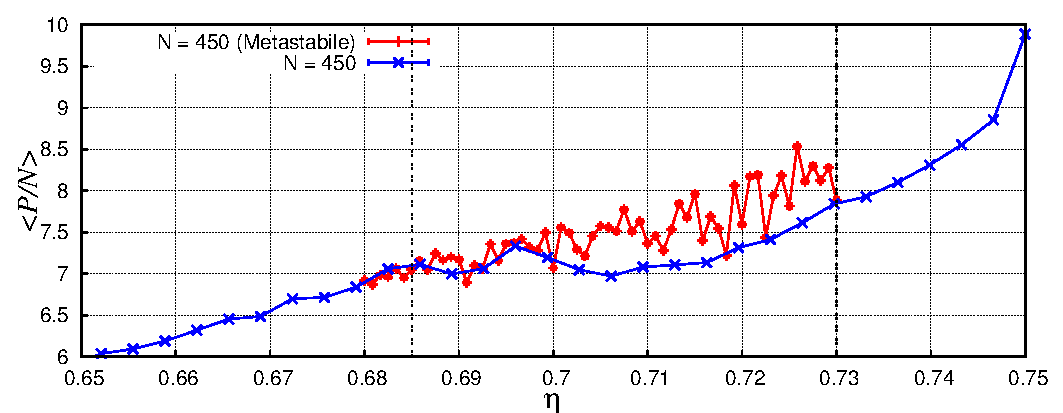
\includegraphics[scale=0.85]{Immagini/Rigide/PvsEta2DZoom}
	\newline \footnotesize{$N= 450$ , $d=2$ , campioni$= 100000$ ,  urti termal=$ 50 \cdot N$}
	\label{fig: PvsEta2D_Zoom}
\end{figure}
\begin{figure}[!ht]
\centering
\caption[Sfere Rigide$/$PvsEta\_3D\_ZonaMeta.cpp]{Ingrandimento sulla zona metastabile( caso 3D ).} 	\vspace{-15pt}
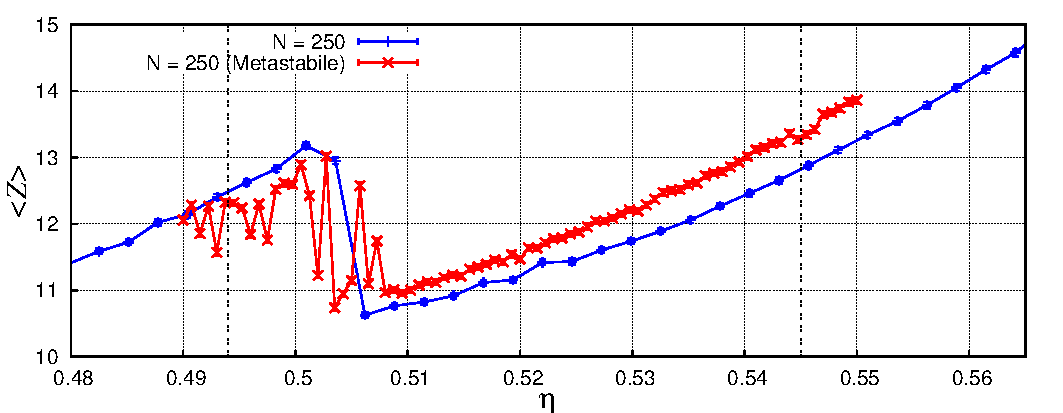
\includegraphics[scale=0.85]{Immagini/Rigide/PvsEta3DZoom}
	\newline \footnotesize{$N= 250$ , $d=3$ , campioni$= 100000$ ,  urti termal=$ 50 \cdot N$}
	\label{fig: PvsEta3D_Zoom}
\end{figure}

In tutte le misurazioni precedenti è stato stimato l'errore tramite il metodo di \emph{Binning} in modo da limitare l'effetto dell'autocorrelazione delle configurazioni temporalmente vicine.

\FloatBarrier 
\subsubsection{Tempi di Collisione e Libero Cammino Medio}
Due quantità che è possibile monitorare per studiare il cambiamento di fase sono il tempo di collisione medio e il libero cammino medio.

  \begin{figure}[h!]\vspace{-10pt}
     \begin{minipage}{0.4\textwidth}
		\begin{flushright}
		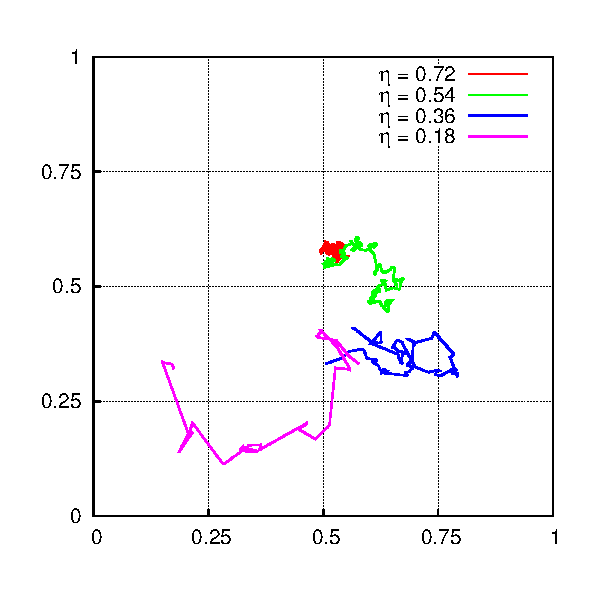
\includegraphics[scale=0.65]{Immagini/Rigide/Lc_2D}
		\end{flushright}
     \end{minipage}\hfill
     \begin{minipage}{0.55\textwidth}
     	\begin{flushleft}
		\caption[Sfere Rigide$/$Preliminari\_Cammino.cpp]{Cammino percorso da una particella durante l'evoluzione di $1 [t]$ .\newline \footnotesize{$N= 450$ , $d=2$ ,  urti termal=$ 20 \cdot N$}}\label{fig: SnapLiberoCammino}
     \end{flushleft}
     \end{minipage}\vspace{-15pt}
  \end{figure}

In un sistema molto denso le particelle tenderanno ad incontrarsi più spesso, in questo caso la frequenza degli urti sarà molto alta e il cammino libero medio tendenzialmente molto basso.

\begin{figure}[htbp]
\centering
\caption[Sfere Rigide$/$Problema2.cpp]{Andamento del tempo di collisione medio in funzione di $\eta$.}\vspace{-15pt}
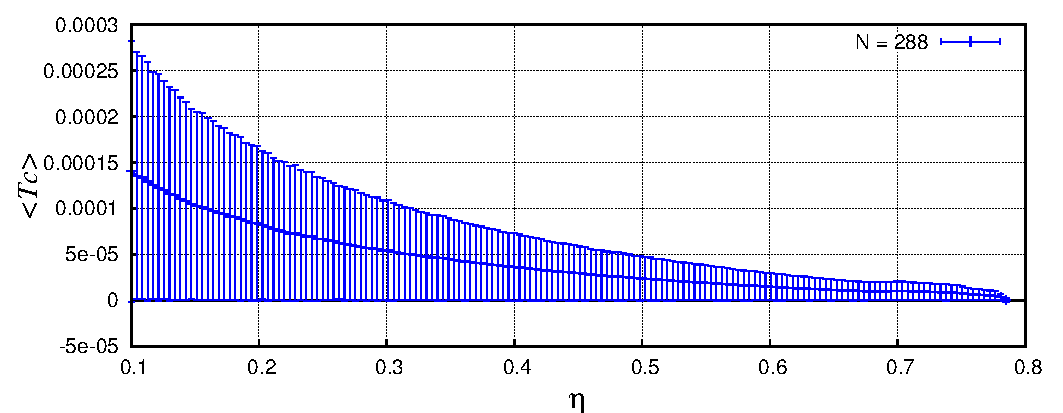
\includegraphics[scale=0.95]{Immagini/Rigide/TcvsEta2D}
	\newline \footnotesize{$N= 450$ , $d=2$ , campioni$= 50\cdot N$ ,  urti termal=$ 50 \cdot N$}
	\label{fig: TcvsEta}
\end{figure}
\begin{figure}[htbp]
\centering
\caption[Sfere Rigide$/$Problema4.cpp]{Andamento del libero cammino medio in funzione di $\eta$.}\vspace{-15pt}
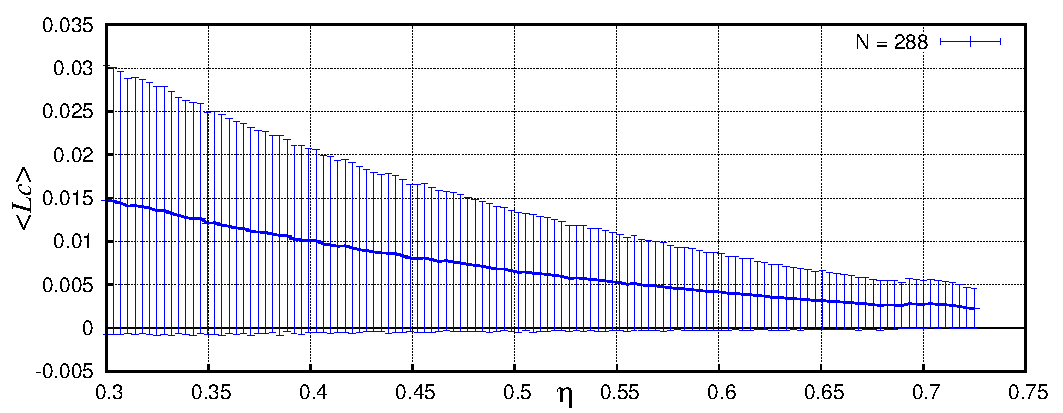
\includegraphics[scale=0.95]{Immagini/Rigide/LcvsEta2D}
	\newline \footnotesize{$N= 450$ , $d=2$ , campioni$= 50\cdot N$ ,  urti termal=$ 50 \cdot N$}
	\label{fig: LcvsEta}
\end{figure}

Nelle figure (\ref{fig: TcvsEta}) e (\ref{fig: LcvsEta}) è possibile osservare come il modello segua l'andamento previsto, le curve presentano una piccola flessione in presenza della zona metastabile ($\eta \simeq 0.7$) dove il sistema oscilla tra stato fluido e stato solido.


\begin{figure}[htbp]
\centering
	\caption[Sfere Rigide$/$Problema3.cpp]{Distribuzione dei tempi di collisione per vari valori di $\eta$.}\vspace{-15pt}
	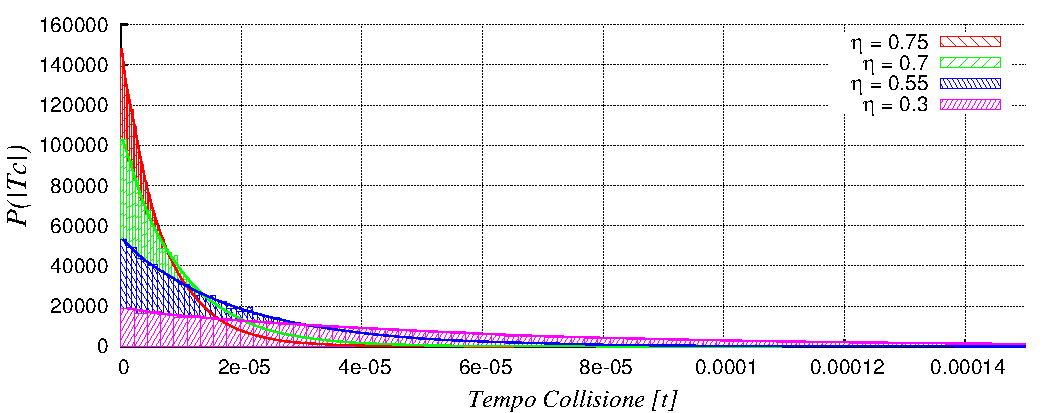
\includegraphics[scale=0.95]{Immagini/Rigide/DistroTc2D}
\newline \footnotesize{$N= 450$ , $d=2$ , campioni$= 50\cdot N$ ,  urti termal=$ 50 \cdot N$}
	\label{fig: DistroTc}
\end{figure}

\begin{figure}[htbp]
\centering
	\caption[Sfere Rigide$/$Problema4\_2.cpp]{Distribuzione dei valori del libero cammino per vari valori di $\eta$.}\vspace{-15pt}
	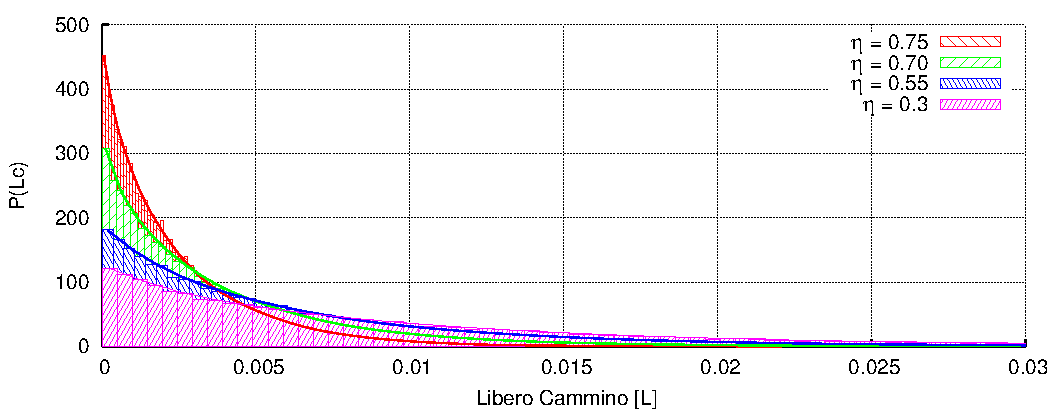
\includegraphics[scale=0.95]{Immagini/Rigide/DistroLc2D}
	\newline \footnotesize{$N= 450$ , $d=2$ , campioni$= 50\cdot N$ ,  urti termal=$ 50 \cdot N$}
	\label{fig: DistroLc}
\end{figure}
Nei grafici precedenti è stato mostrato l'andamento degli osservabili medi, studiando la distribuzione di probabilità dei valori raccolti è possibile determinare il modo in cui i valori campioni si dispongono attorno a a tale valore medio.
Nelle figure (\ref{fig: DistroTc}) e (\ref{fig: DistroLc}) è mostrato l'andamento di tali distribuzioni di probabilità. Si può notare come la distribuzione risulti estremamente piccata attorno al valore medio nel caso della fase solida e come invece, nella fase liquida e in quella metastabile, i campioni tendano a distribursi in modo quasi uniforme in un largo intervallo di valori .

Il risultato non è sorprendente, la collisione costituisce un evento \emph{pseudo-casuale}( il sistema è classico quindi deterministico).
Mentre in un sistema fluido tale evento può avvenire ad intervalli di tempo molto diversi, in un sistema solido, dove ogni particella è incastrata in un reticolo, le particelle non hanno lo spazio materiale per fluire e urteranno necessariamente con immediatamente vicine. 
In altre partole la mancanza di spazio determinata dall'elevata densità non da la possibilità alle particelle limitrofe di aprire un varco che consenta alla particelle di viaggiare liberamente.
\FloatBarrier 
Unendo questi dati ai risultati ottenuti nel capitolo precedente è possibile determinare la natura delle transizioni di fase al variare della frazione d'impacchettamento:
\begin{center}
\begin{tabular}{|c|c | c | c |}
\hline
		 & Fase Liquida & Fase Metastabile & Fase solida	\\
\hline
	$2D$ & $\eta < 0.685$ & $0.685 <\eta < 0.735$ & $\eta > 0.735$ \\
\hline
	$3D$ & $\eta < 0.49$ & $0.49 <\eta < 0.55$ & $\eta > 0.55$ \\
\hline
\end{tabular}
\end{center}

\FloatBarrier 
\subsubsection{Studio della Diffusione: spostamento quadratico medio.}
Un ulteriore osservabile che può essere utile per distinguere le fasi del sistema è lo spostamento quadratico medio.

  \begin{figure}[h!]\vspace{-10pt}
     \begin{minipage}{0.4\textwidth}
		\begin{flushright}
			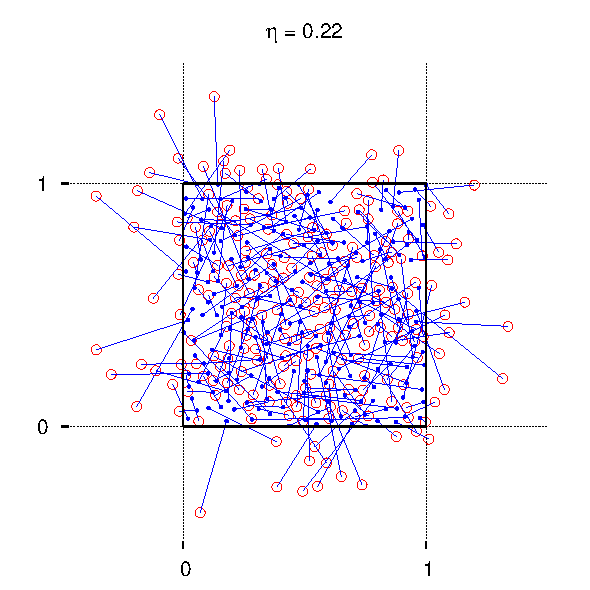
\includegraphics[scale=0.55]{Immagini/Rigide/Eta4_2D}
		\end{flushright}
     \end{minipage}\hfill
     \begin{minipage}{0.4\textwidth}
     	\begin{flushleft}
		\caption[Sfere Rigide$/$Preliminari\_Diffusione.cpp]{Immagine della diffusione del sistema dopo $1 [t]$ . \newline \footnotesize{$N= 242$ , $d=2$ ,  urti termal=$ 20 \cdot N$}}
     \end{flushleft}
     \end{minipage}\vspace{-10pt}
  \end{figure}
Anche in questo caso le due regioni di $\eta$ individuate in precedenza mostrano le proprietà attese teoricamente.

\begin{figure}[!htbp]
\caption[a) Sfere Rigide$/$Problema5\_0.cpp $\quad / \quad$b) Sfere Rigide$/$Problema7\_0.cpp]{Andamento dello spostamento quadratico medio in funzione del tempo di evoluzione per vari valori di $\eta$.}\vspace{-10pt}
		\begin{subfigure}[b]{\textwidth}
          	\begin{center}
	\caption[Sfere Rigide$/$Problema5\_0.cpp]{( caso 2D )}\vspace{-10pt}
	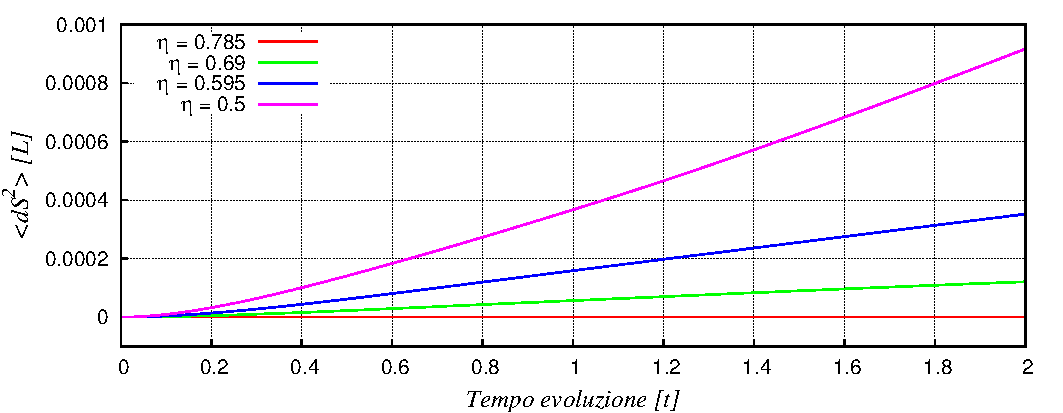
\includegraphics[scale=0.75]{Immagini/Rigide/dSquadvsDt_2D}
	\newline \footnotesize{$N= 450$ , $d=2$ , campioni$= 2000$,  urti termal=$ 20 \cdot N$} 
	\label{fig: dSquadvsDt_2D}	
          	\end{center}
        \end{subfigure}%
  	\medskip
  	
        \begin{subfigure}[b]{\textwidth}
            \begin{center}           
			\caption[Sfere Rigide$/$Problema7\_0.cpp]{ \centering ( caso 3D )}\vspace{-10pt}	
			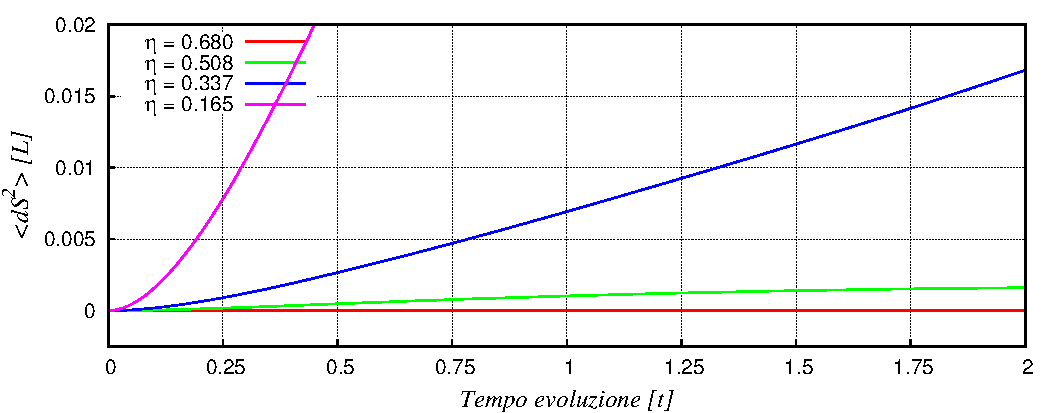
\includegraphics[scale=0.75]{Immagini/Rigide/dSquadvsDt_3D}
			\newline \footnotesize{$N= 250$ , $d=3$ , campioni$= 2000$,  urti termal=$ 50 \cdot N$}
			\label{fig: dSquadvsDt_3D}
			\end{center}
        \end{subfigure}
\end{figure}
Nelle  figure (\ref{fig: dSquadvsDt_2D}) e (\ref{fig: dSquadvsDt_3D}) è mostrato l'andamento dalla distanza quadratica media percorsa dalle particelle del sistema in un intervallo di tempo di diffusione  fisso. 
Si può notare come nella fase liquida lo spostamente quadratico medio cresca linearmente con l'aumentare del tempo di diffusione mentre , nella fase solida, rimanga costante attorno allo spostamento di oscillazione termica medio. 

\FloatBarrier 
Lo studio dell'andamento dello spostamento quadratico medio( in un intervallo di tempo fissato) al variare della densità del sistema fornisce un altro criterio per mostrare il camibiamento di fase subito dal sistema.
Dalle figure (\ref{fig: dSquadvsEta_2D}) e (\ref{fig: dSquadvsEta_3D}) si nota come la distanza (quadratica) media percorsa dalle particelle nel loro moto di diffusione decada con l'aumento della frazione d'impacchettamento in accordo con l'aumento della frequenza della collisioni che hanno l'effetto di deviare la traiettoria rettilinea della molecola.

\begin{figure}[!htbp]
\caption[a) Sfere Rigide$/$Problema5\_1.cpp $\quad / \quad$b) Sfere Rigide$/$Problema7\_1.cpp]{Andamento dello spostamento quadratico medio in $0.5[t]$ di evoluzione in funzione di $\eta$.}\vspace{-10pt}
		\begin{subfigure}[b]{\textwidth}
          	\begin{center}
	\caption[Sfere Rigide$/$Problema5\_1.cpp]{( caso 2D )}\vspace{-15pt}
	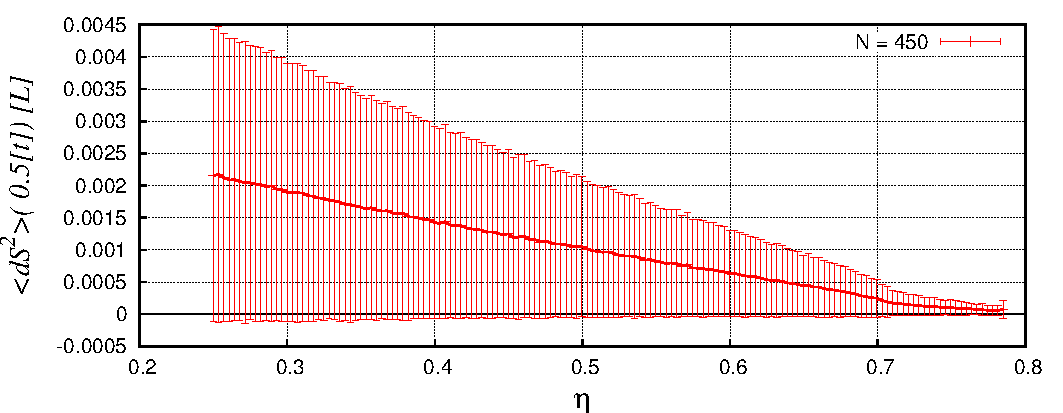
\includegraphics[scale=0.85]{Immagini/Rigide/dSquadvsEta_2D}
	\newline \footnotesize{$N= 450$ , $d=2$ , campioni$= 500$ per particella,  urti termal=$ 20 \cdot N$}
	\label{fig: dSquadvsEta_2D}
          	\end{center}
        \end{subfigure}%
  	\medskip
  	
        \begin{subfigure}[b]{\textwidth}
            \begin{center}           
	\caption[Sfere Rigide$/$Problema7\_1.cpp]{( caso 3D )}\vspace{-15pt}
	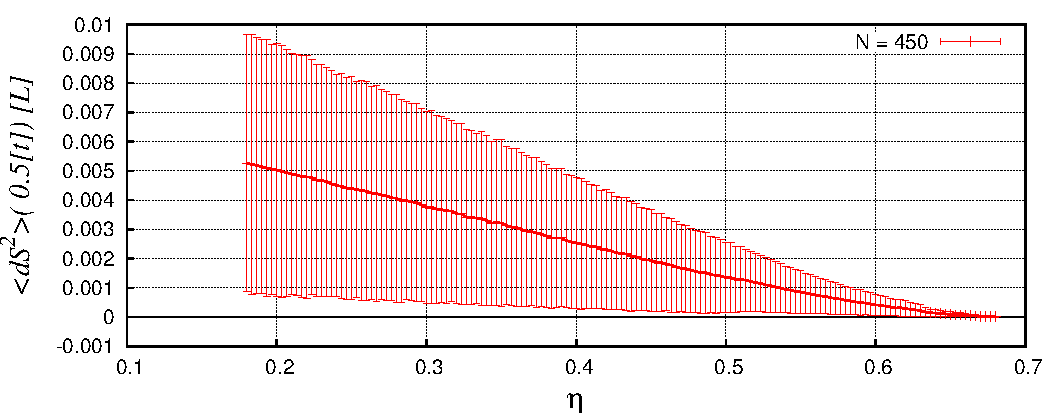
\includegraphics[scale=0.85]{Immagini/Rigide/dSquadvsEta_3D}
	\newline \footnotesize{$N= 250$ , $d=3$ , campioni$= 500$ per particella,  urti termal=$ 100 \cdot N$}
	\label{fig: dSquadvsEta_3D}
			\end{center}
        \end{subfigure}
\end{figure}



\FloatBarrier 
\subsubsection{Studio della Diffusione: Funzione di Distribuzione Radiale}
Un'altro indicatore dell'effettivo comportamento solido-liquido manifestato del sistema a sfere rigide è fornito dalla fuzione di distribuzione radiale al tempo t $g_t(r)$.
\newline
L'andamento della funzione mostrato nelle figure (\ref{fig: DistrodS_2D}) e (\ref{fig: DistrodS_3D}) è esattamente quello previsto nel capitolo \ref{cap: Simulazione in Generale}.
\newline
Nelle figure è anche possibile notare come nella fase metastabile due valori (curve blu e verde), molto simili ma diversi, possano dare distribuzioni completamente diverse a secondo di quale sia la configurazione a partire da cui vengono inizializzati.

\begin{figure}[htbp]
\centering
		\caption[Sfere Rigide$/$Problema5\_2.cpp]{Funzione di distribuzione radiale del sistema dopo $250[t]$ di evoluzione.}\vspace{-15pt}
		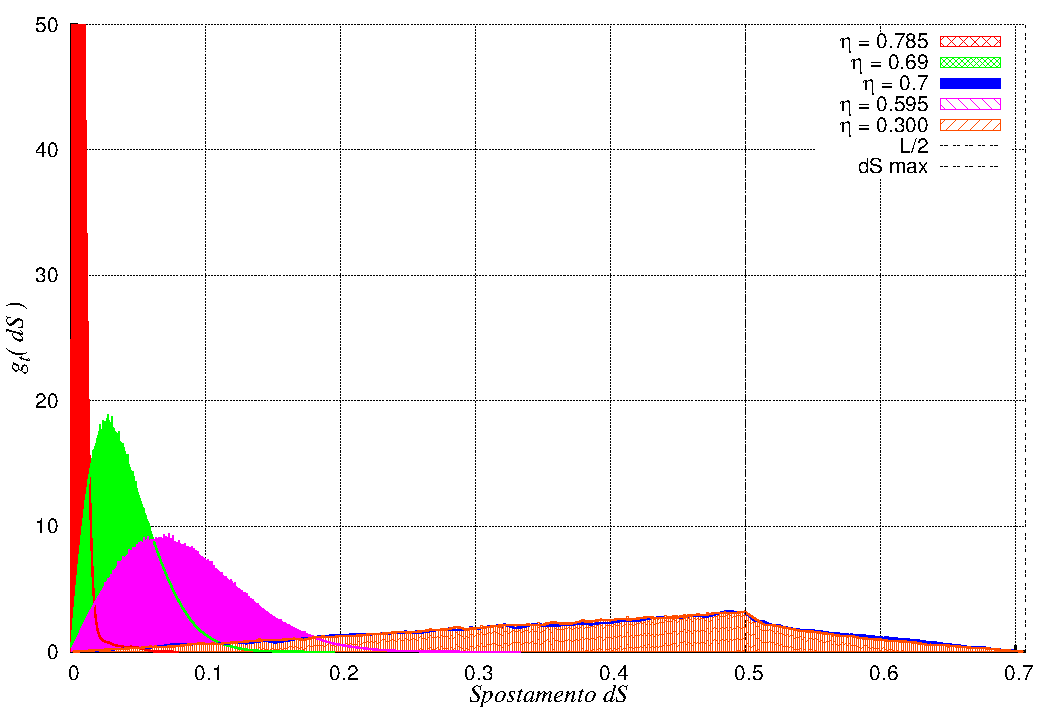
\includegraphics[scale=1]{Immagini/Rigide/DistrodS_2D}
		\newline \footnotesize{$N= 450$ , $d=2$ , campioni$= 500$ per particella,  urti termal=$ 150 \cdot N$}
	\label{fig: DistrodS_2D}

\centering
	\caption[Sfere Rigide$/$Problema7\_2.cpp]{Funzione di distribuzione radiale del sistema dopo $10[t]$ di evoluzione.}\vspace{-15pt}
	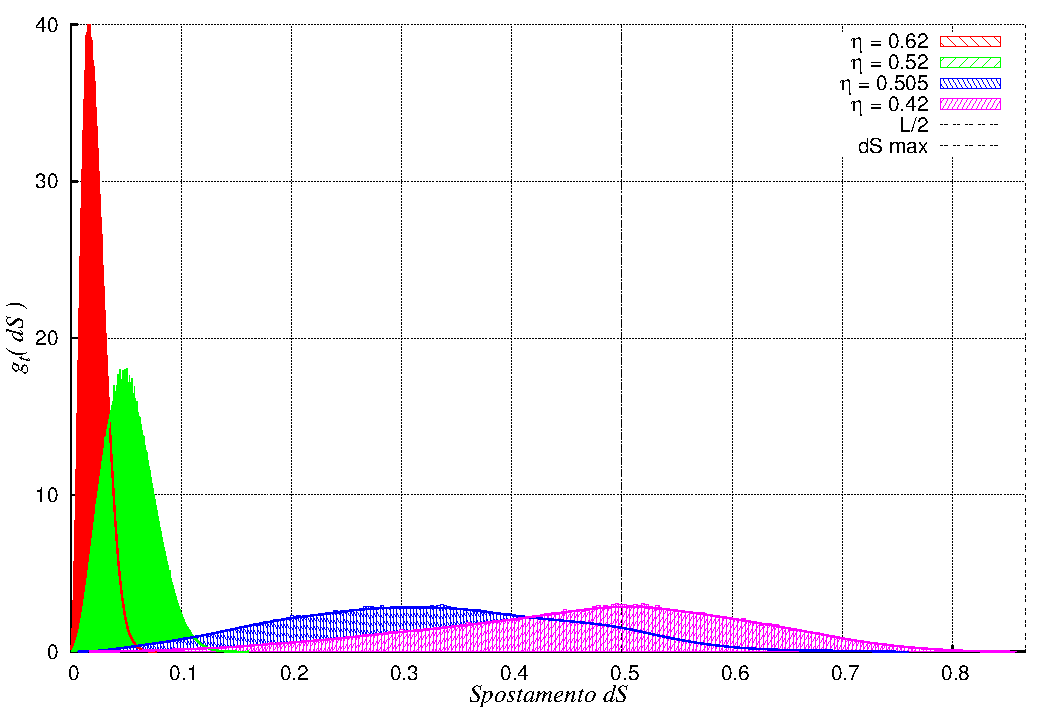
\includegraphics[scale=1]{Immagini/Rigide/DistrodS_3D}
	\newline \footnotesize{$N= 250$ , $d=3$ , campioni$= 800$ per particella,  urti termal=$ 150 \cdot N$}
	\label{fig: DistrodS_3D}
\end{figure}



\FloatBarrier 
\subsection{Studio del limite termodinamico}
Nella figura (\ref{fig: Limite Termo}) è mostrato il valore di $\langle Z-1 \rangle$  calcolato per sistemi caratterizzati dalla stessa frazione di impacchettamento ma simulati con diverso numero di particelle.

\begin{figure}[htbp]
\centering
	\caption[Sfere Rigide$/$Problema8.cpp]{Andamento del parametro Z in funzione di $N$. Limite Termodinamico }\vspace{-10pt}
	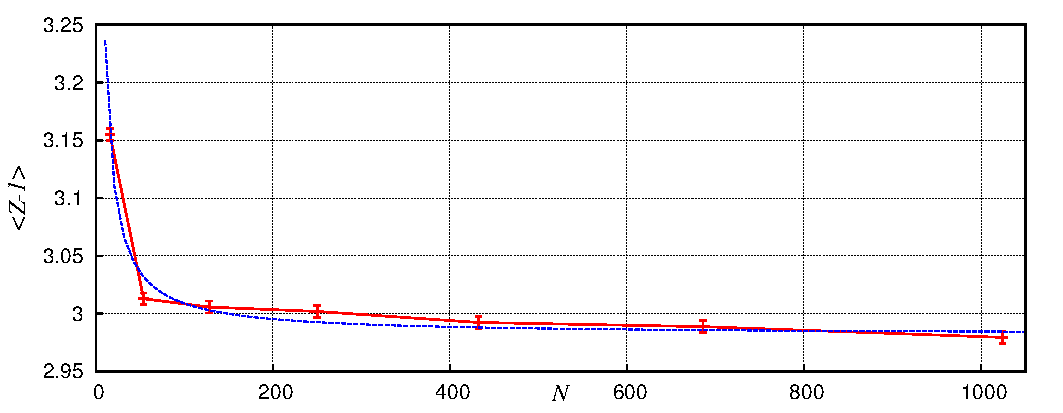
\includegraphics[scale= 1]{Immagini/Rigide/termPvsN3D}
	\newline\footnotesize{ $d=3$ , campioni$= 500000$,  urti termal=$ 500000$}
	\label{fig: Limite Termo}
\end{figure}

Eseguendo un fit dei valori calcolati rispetto ad un andamento del tipo:
\begin{equation}\label{eq: limiteTermo}
 (Z-1) = A + \dfrac{B}{N}
\end{equation}
si ottengono le seguenti stime per i parametri della funzione:
\begin{center}
\begin{tabular}{|c c r c l |}
\hline
	A	 & $=$ & $ 2.98 $ & $\pm$ & $0.01 $	\\
	B	 & $=$ & $ 2.70$ & $\pm$ & $0.2 $	\\
\hline
\end{tabular}
\end{center}

Calcolando il limite per $N\rightarrow \infty$ si ottiene una stima del fattore di comprimibilità al limite termodinamico pari a: 
\begin{displaymath}
Z_{\textrm{TD}} (\eta = 0.3) = 3.98 \pm 0.01
\end{displaymath}


\clearpage
\newpage
%/\/\/\/\/\/\/\/\/\/\/\/\/\/\/\/\/\/\/\/\/\/\/\/\/\/\/\/\/\/\/\/\/\/\/\/\/\/\/\/\/\/\/\
\section{Sfere Soffici}\label{Soffici}
In un generico modello a \emph{Sfere Soffici} il potenziale di interazione tra le particelle è una funzione continua della distanze.
\newline
Il potenziale più adatto alla descrizione delle interazioni intermolecolari è quello proposto su base fenomenologica da Lennard-Jones, definito dall'equazione:
\begin{equation}
u(r) = 4\epsilon \biggr[\big(\frac{\sigma}{r} \big)^{12} - \big(\frac{\sigma}{r} \big)^6 \biggr]
\end{equation}
dove la costante $\epsilon$ rappresenta il minimo dell'energia e $\sigma$ la distanza di annullamento del potenziale.
\newline
I due esponenti sono stati scelti attraverso un criterio empirico, devono essere tali da determinare una forza di attrazione tra particelle distanti e una bariera repulsiva a distanze piccole.

	\begin{figure}[htbp]
		\centering
		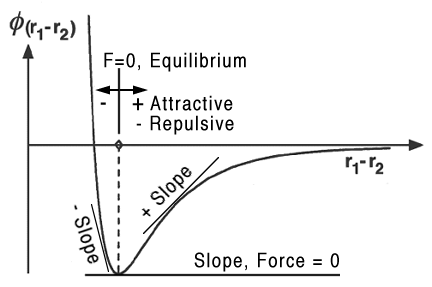
\includegraphics[scale=0.5]{Immagini/LJ}
		\caption[Potenziale di L.-J.]{Andamento del potenziale di Lennard-Jones.}\label{fig: LJunCut}
	\end{figure}




\FloatBarrier 
\subsection{Metodi Numerici e Simulazione Computazionale}
Come nel caso precedente, prima di passare allo studio del calcolo numerico della simulazione, è necessario scegliere un sistema di unità di misura caratteristico del modello.

\paragraph{Unità di Misura del sistema}
\begin{itemize}
\item[-] \underline{Massa}: $[M]=m=1$ 
\newline Tutte le particelle sono identiche è la loro massa fornisce l'unità di misura più ovvia.

\item[-] \underline{Lunghezza}: $[L]=\sigma=1$ 
\newline Il lato della scatola verrà genralmente misurato in unità di $\sigma$ (diametro della particella).

\item[-] \underline{Energia}: $[E]=\epsilon=1$ 
\newline Nell'espressione del potenziale è presente una scala naturale di energia data dalla costante $\epsilon$.
\end{itemize}
In queste unità di misura gli osservabili definiti nel capitolo (\ref{cap: Intro dinamica}) verrano espressi nel seguente modo:
\begin{eqnarray}
	\dfrac{kT}{\epsilon}  = T \\
	\dfrac{U}{N \epsilon} = U \\
	\dfrac{P \rho}{kT}	  = Z = 1 + P^{*}
\end{eqnarray}

\FloatBarrier 
\subsubsection{Taglio del potenziale}
Per simulare l'evoluzione del sistema è necessario conoscere la forza totale applicata su ogni particella che lo compone.
L'interazione tra sfere soffici è a 2 corpi e a lungo range, partanto sarà sarà necessario, in linea di pricipio, calcolare il contributo di interazione generato da ogni coppia di particelle, quindi $N(N-1)$ contributi in totale.

Come è visibile dalla figura (\ref{fig: LJunCut}, la forza diventa rapidamente molto piccola al crescere della distanza, si può quindi avere un notevole aumento nell'efficienza del calcolo trascurando le interazioni che avvengono a distanze troppo grandi.\newline
In altre parole è possibile considere un potenziale troncato del tipo:

\begin{displaymath}
	u_c(r) = 
	\begin{cases}u(r) & r \leq r_c\\
	0 & r > r_c \end{cases}
\end{displaymath}

Un potenziale di questa forma determina un troncamento anche per la forza associata con la conseguenza che 
ogni volta che una particella supera la distanza $r_c$ questa acquista un piccolo impulso.
Queste variazioni discontinue dei momenti determinano delle oscillazioni nell'energia totale del sistema annullando la conservazione dell'energia prevista per i sistemi isolati.

Quindi l'espressione troncata non rappresenta una buona approssimazione del potenziale iniziale.
E' necessario introdurre un'ulteriore correzione per assicurare la conservazione dell'energia definita dall'equazione:
\begin{equation}\label{eq: forza usata}
	F_{s}(r) = 
	\begin{cases}
	 -\dfrac{d}{dr} u(r) - \biggr(\dfrac{d}{dr} u(r)\biggr)\Biggr\vert_{r_c} & r \leq r_c\\
	0 & r > r_c 
	\end{cases}
\end{equation}
che determina un potenziale del tipo:
\begin{equation}\label{eq: potenziale usato}
	u_{s}(r) = 
	\begin{cases} u(r) - u(r_c) -[r -r_c]\biggr(\dfrac{d}{dr} u(r)\biggr)\Biggr\vert_{r_c} & r \leq r_c\\
	0 & r > r_c \end{cases}
\end{equation}
che sostanzialmente esprime una forza d'interazione troncata e traslata in modo da annullarsi alla distanza $r_c$.

L'andamento delle nuove espressioni della forza e dell'interazione è visibile nella figura (\ref{fig: LJCut}), dal grafico si può notare come la nuova forma alterata non sia estremamente simile dall'espressione iniziale.

	\begin{figure}[htbp]
		\centering
		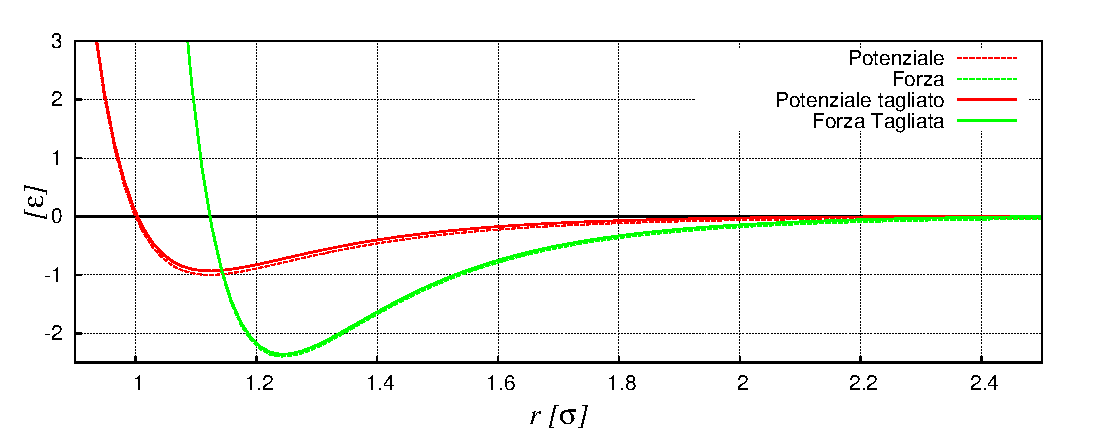
\includegraphics[scale=0.95]{Immagini/Soffici/potenziale}
		\caption[Potenziale di L.-J. tagliato]{Andamento del potenziale di Lennard-Jones tagliato e traslato e della forza corrispondente.}\label{fig: LJCut}
	\end{figure}

Tipicamente si sceglie come valore di taglio la distanza $r_c = 2.5 \sigma$ che corrisponde a trascurare valori della forza dell'ordine di $F(r_c) = -0.039 \epsilon / \sigma$.

\FloatBarrier 
\subsubsection{Metodo della lista dei vicini}
La parte della dinamica che richiede il maggiore sforzo computazionale è il calcolo della forza d'interazione, il metodo del potenziale troncato permette di migliorare l'efficienza di questa fase ma richiede in ogni caso di calcolare la distanza tra tutte le possibile coppie di particelle in ogni istante dell'evoluzione ( e in un sistema con bordo periodico tale misura non è immediata).

La velocità del calcolo numerico del sistema può essere ulteriormente raffinata introducendo la lista dei vicini.
Questa lista tiene conto di tutte le coppie di particelle che distano tra loro meno di $r_L \simeq r_c +0.3\sigma$, in questo funge da guida indicando quali coppie di particelle sono sufficientemente vicine da determinare una forza d'interazione non trascurabile.\newline
La distanza $r_L$ di "vicinanza" scelta è maggiore della distanza $r_c$ di "taglio", in questo modo la lista tiene traccia non solo delle particelle a distanza sufficientemente piccola da determinare un'interazione ma anche le particelle che entreranno nel raggio d'interazione in un certo intervallo di tempo $\check{T}$. \newline
Il vantaggio di tale prescrizione è di rendere la lista dei vicini valida per più di un evoluzione temporale, in tal caso non sarà necessario aggiornare la lista( e calcolare le distanze) ad ogni istante ma basterà farlo ogni $\check{T}$, intervallo di tempo pari a :
\begin{displaymath}
\check{T} \cdot \langle \vert \vec{v} \vert \rangle \simeq r_L - r_c = 0.3 \sigma
\end{displaymath}
corrispondende al tempo medio necessario ad una particella per percorrere la distanza $r_L - r_c$.

\FloatBarrier 
\subsubsection{Algoritmo di Evoluzione del sistema}
L'introduzione dell'espressione approssimata per l'interazione non altera le leggi che regolano l'evoluzione dinamica del sistema, restano, in ogni caso, da risolvere le equazioni differenziali del moto.
Per un sistema dotato di un grande numero di particelle come quello in esame la soluzione esatta del sistema di equazioni di Newton è totalmente improponibile.
L'unico approccio possibile è quello di affidarsi alle soluzione approssimate fornite dai metodi del calcolo numerico.

Esistono diversi metodi per il calcolo numerico delle soluzioni di equazioni differenziali, in generale nessuno di essi è in grado di calcolarla nel complesso ma solo di fornire una soluzione approssimata punto per punto risolvendo il problema di Cauchy su intervalli discreti consecutivi.
\newline
Pertanto sarà essenziale suddividere il tempo d'evoluzione in passi discreti, in questo articolo l'intervallo di tempo fondamentale è stato scelto pari a $t_{step} = 0.001 [t]$.
\medskip

L'algoritmo che è stato scelto per la simuluzione è il metodo di \emph{Velocity Verlet}( per il calcolo della soluzione delle equazioni del moto) che implementato congiuntamente alla tecnica della lista dei vicini determina il seguente ciclo per il calcolo del passo d'evoluzione del sistema:
\medskip
\begin{figure}[!htbp]
\begin{tikzpicture}[node distance = auto]
    % Place nodes
    \node [block_med] (1) {Evoluzione delle posizioni di ogni particella di un passo $\Delta t = t_{step}$ \newline \footnotesize $$\vec{r_i}(t_0) \mapsto \vec{r_i}(t_0 + \Delta t) = \vec{r_i}(t_0) + \vec{v_i}(t_0) \cdot \Delta t + \dfrac{1}{2} \vec{a_i}(t_0) \cdot \Delta t^2$$};
    \node [block_med, below of=1,node distance=2.25cm] (2) {Calcolo delle velocità a mezzo passo. \newline \footnotesize $$ \vec{v_i}(t_0 + \Delta t/2) = \vec{v_i}(t_0) + \dfrac{1}{2} \vec{a_i}(t_0) \cdot \Delta t$$ };
    \node [block_med, below of=2,node distance=2.55cm] (3) {Ricalcolo delle accelerazioni delle particelle. \newline \footnotesize $$\vec{a_i}(t_0) \mapsto \vec{a_i}(t_0 + \Delta t)=
     \overbrace{\sum_{i}^{} \sum_{j>i}^{}}^{j \in \text{Vicini}(i)} 
     F_s(\bar\vec{r_i}(t_0 + \Delta t) -\vec{r_j}(t_0 + \Delta t \bar )$$}; %\textrm($j$ vicino a $i$)    
    \node [decision, right of=3,node distance=9.25cm] (5) {\footnotesize Riaggiornamento della lista dei vicini ogni $10$ passi $\Delta t$.};        
    \node [block_med, below of=3,node distance=2.75cm] (4) {Evoluzione delle velocità in accordo con le accelerazioni aggiornate \newline \footnotesize $$\vec{v_i}(t_0) \mapsto \vec{v_i}(t_0 + \Delta t) = \vec{v_i}(t_0 + \Delta t/2) + \dfrac{1}{2}\vec{a_i}(t_0+\Delta t)\cdot \Delta t$$};
 
    % Draw edges
    \path [line] (1) -- (2);
    \path [line] (2) -- (3);
    \path [line] (3) -- (4);
    \path [line] (4) -| (5);
    \path [line] (5) |- (1);
\end{tikzpicture}
\end{figure}

\FloatBarrier 
\subsubsection{Implementazione computazionale dell'algoritmo}
Per simulare questo sistema verrà utilizzata la programmazione ad oggetti del linguaggio C++.
La logica usata per il programma è la stessa sfrutta per la simulazione del sistema a sfere rigide.
\newline
Si definire la classe \Cls{sistema\_soffice()} dotata degli attributi necessari a descrivere lo stato microscopico del sistema:
\begin{itemize}
\item 3 array di vettori per memorizzare posizione, velocità e accelerazione di tutte le particelle costituenti il sistema.

\item 2 array per memorizzare la \emph{lista dei vicini} associata allo stato del sistema. Il vettore \cd{NPoint} contiene nell'ingresso $i$ l'indice del vettore \cd{List} dopo di cui comincia l'elenco delle particelle vicine alla particella $i$. Il vettore \cd{List} viene costruito testando in modo sequenziale tutte le coppie $($ $P[i]$, $P[j]$ $)_{j>i}$ e salvando tutti gli indici $j$ relativi a coppie "vicine" secondo la definizione del paragrafo precedente.

\item 5 variabili \emph{double} per contenere le variabili $r_c$, $r_L$,$\sigma$,$\epsilon$ e L. 2 varibili \emph{int} per salvare il numero di particelle e la dimensione spaziale della simulazione.

\end{itemize}
%\medskip\newline
Il costruttore della classe costituirà la fase di \emph{inizializzazione} dell'algoritmo, ovvero salverà le posizioni disponendole nel reticolo bcc più piccolo in grando di contenerle tutte, attribuirà velocità iniziali casuali riscalandole a Momento totale nullo, inizializza la lista dei vicini e calcola le accelerazioni per la prima volta.
Le variabili necessarie per inizializzare il sistema, argomenti della funzione costruttore, saranno la dimensione spaziale $d$, la densità del sistema e il numero $N$ di particelle contenute.
\medskip\newline
Il metodo \cd{evoluzione()} è il cardine della simulazione, questa funzione fornisce l'evoluzione temporale del sistema di un $t_{step}$ sfruttando la tavola dei vicini precedentemente calcolata. I metodi che calcolano passi d'evoluzione consecutivi provvederanno a ricalcolare la lista dei vicini ogni 10 $t_{step}$
\medskip\newline
La fase di \emph{termalizzazione} si ottiene applicando il metodo di evoluzione un numero di volte sufficiente a realizzare la distribuzione di Maxwell-Boltzman per le velocità.
\medskip\newline
Similmente la fase di \emph{produzione} si realizza intervallando la raccolta di osservabili istantanei sulla configurazione occupata dal sistema all'evoluzione temporale necessaria per ottenere un'altra configurazione sufficientemente scorrelata dalla prima.
\medskip\newline
Per ottenere rapidamente una successione di sistemi inizializzati con un diverso numero di particelle e valore di densità viene usato il metodo \cd{rinizializzazione()}. Tale metodo prende in ingresso i nuovi valore di $N$ e di $rho$ (minori di quelli precedenti), ricalcola il lato della scatola, espande proporzionalmente i vettori posizione e ricalcola la lista dei vicini di conseguenza.



\FloatBarrier 
\subsection{Caratteristiche dell'algoritmo di Simulazione}
\begin{figure}[htbp]
		\caption[Sfere Soffici$/$Preliminari\_Snap2D.cpp]{Immagini del sistema 2D termalizzato a diversi valori di densità e Temperatura (In alto a sinistra è visibile la configurazione inziale prima dell'evoluzione temporale).}\vspace{-15pt}
        \begin{subfigure}[b]{0.5\textwidth}
                \centering
                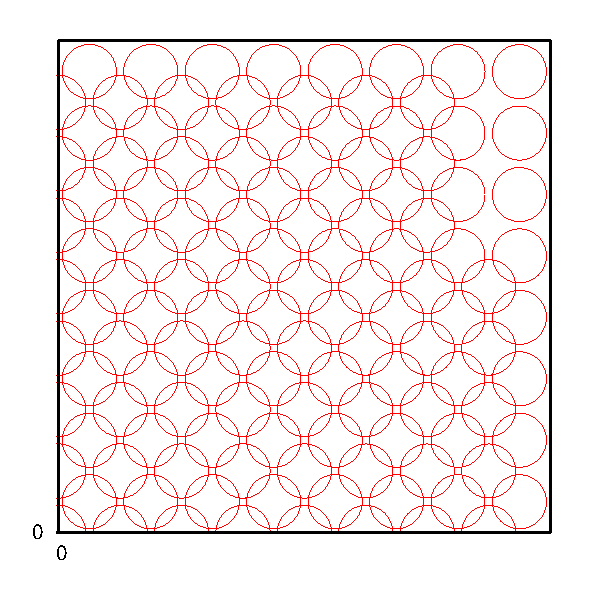
\includegraphics[width=0.85\textwidth]{Immagini/Soffici/SnapSolidoCompresso_Inizio_2D}
        \end{subfigure}%
        ~ %add desired spacing between images, e. g. ~, \quad, \qquad etc. 
          %(or a blank line to force the subfigure onto a new line)
        \begin{subfigure}[b]{0.5\textwidth}
                \centering
                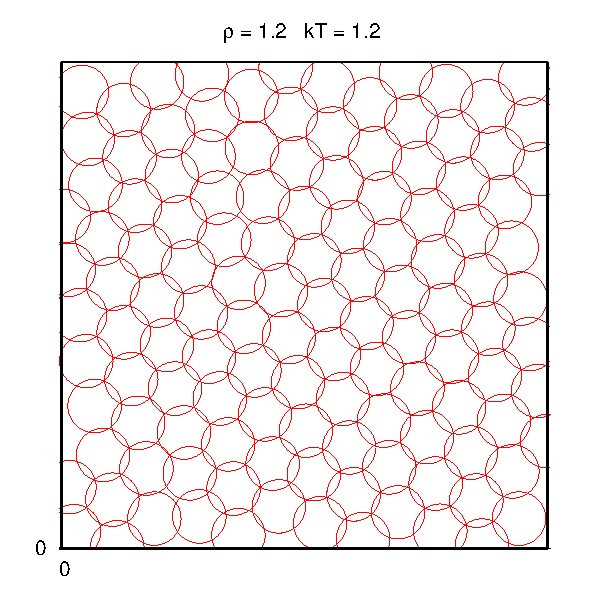
\includegraphics[width=0.85\textwidth]{Immagini/Soffici/SnapSolidoCompresso_2D}
        \end{subfigure}
        ~ %add desired spacing between images, e. g. ~, \quad, \qquad etc. 
          %(or a blank line to force the subfigure onto a new line)

        \begin{subfigure}[b]{0.5\textwidth}
                \centering
                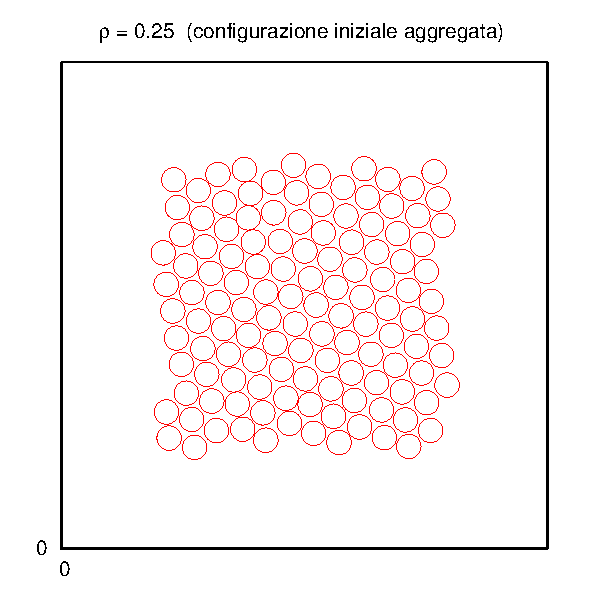
\includegraphics[width=0.85\textwidth]{Immagini/Soffici/SnapSolidoFreddo_Inizio_2D}
        \end{subfigure}
         \begin{subfigure}[b]{0.5\textwidth}
                \centering
                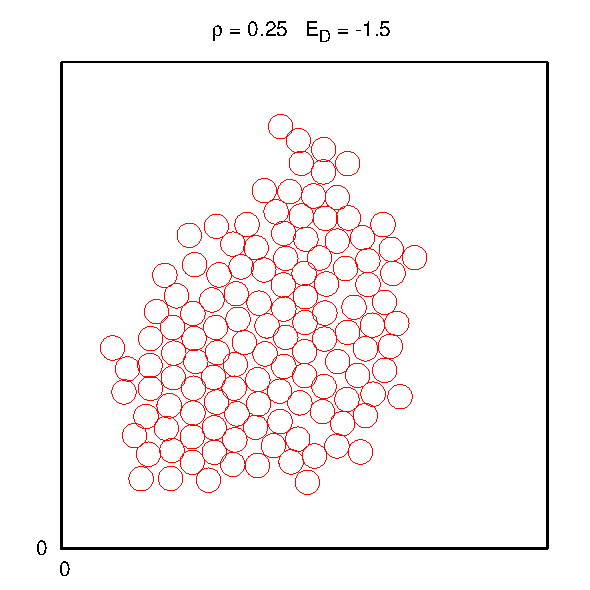
\includegraphics[width=0.85\textwidth]{Immagini/Soffici/SnapSolidoFreddo_2D}
        \end{subfigure}
		
        \begin{subfigure}[b]{0.5\textwidth}
                \centering
                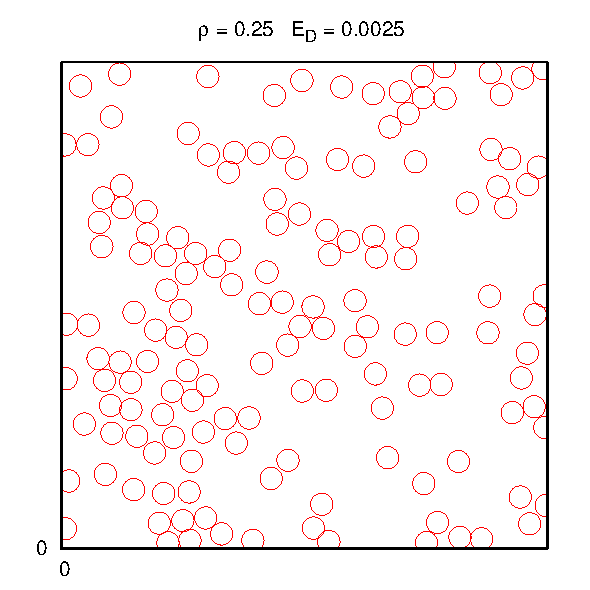
\includegraphics[width=0.85\textwidth]{Immagini/Soffici/SnapSolidoFreddo_2D_Nuclea}
        \end{subfigure}
         \begin{subfigure}[b]{0.5\textwidth}
                \centering
                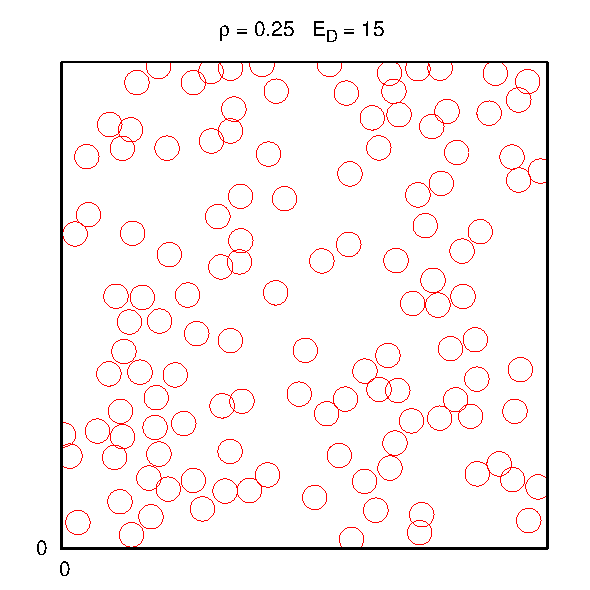
\includegraphics[width=0.85\textwidth]{Immagini/Soffici/SnapLiquido_2D}
        \end{subfigure}
		
		 \centering  \footnotesize{$N= 125$ , $d=2$ , N passi Termalizzazione =$ 500000 $}
		\label{fig: snap2d_soft}
\end{figure}
Nella figura (\ref{fig: snap2d_soft}) sono mostrate delle istantantanee delle configurazioni del sistema a sfere soffici termalizzato a diversi valori delle variabili Termodinamiche che certificano la presenza di una transizione di fase solido-liquido anche per questo modello.
Similmente a quanto accadeva per le sfere rigide il sistema presenta un congelamento di natura geometrica infatti per elevati valori di densità le molecole sono vincolate in un reticolo regolare per via della divergenza infinita del potenziale a brevi distanze (prime 2 figure).

Se l'energia media delle particelle è sufficientemente bassa, la presenza di forze attrattive determina la solidificazione del sistema anche in condizioni di bassa densità.
L'algoritmo usato per la termalizzazione, che consiste in una successione di passi evolutivi intervallati dal riscalamento delle velocità del sistema ad un valore di temperatura( quindi energia cinetica) controllato, non è il procedimento ideale per mostrare questo tipo di transizione.
Nel caso in cui si cerchi di far solidificare un sistema molto rarefatto saranno necessari numerosi passi evolutivi affinchè le particelle, estremamente rallentate dall'abbassamento di temperatura, riescano ad avvicinarsi a sufficienza da aggregarsi e dare il via alla nucleazione.

L'immagine ottenuta precedentemente( ultime 4 figure) invece è stata realizzata a partire da una configurazione ordinata posta in un volume ampio( in modo da diminuire la densità totale), non è in grado di mostrare la solidificazione ma dimostra come il sistema rimanga aggregato in un regione densa in condizione di bassa temperatura sofficiente da non permettere alle molecole di fuoriuscire dai pozzi di potenziale generati dalla sovrapposizione di tutte le interazioni.
La simulazione riesce però a mostrare corrattamente l'evaporazione di questa struttura densa con il riscaldamento del sistema.

\FloatBarrier 
\subsubsection{Tempo di esecuzione}
Il parametro principale che regola il tempo macchina richiesto dalla simulazione di un singolo step di evoluzione del sistema è la dimensione della lista dei vicini. 
Tale lunghezza dipende principalmente da 3 parametri( specifici della simulazione) il numero $N$ di particelle, la densità del sistema $\rho$ e la dimensione spaziale $d$.
Nelle figure (\ref{fig: T_Esec_Confronto_D Soffici}) e (\ref{fig: T_Esec_Confronto_rho Soffici}) è mostrato l'andamento del tempo di esecuzione medio di uno step evolutivo in fuzione del numero $N$ di particelle simulate e per vari valori di densità $\rho$.

	\begin{figure}[htbp]
		\centering
		\caption[Sfere Soffici$/$Preliminari\_TempoEsecuzione.cpp]{Andamento del tempo di esecuzione in funzione del numero di particelle simulate e della Dimensione Spaziale.}\label{fig: T_Esec_Confronto_D Soffici}\vspace{-15pt}
		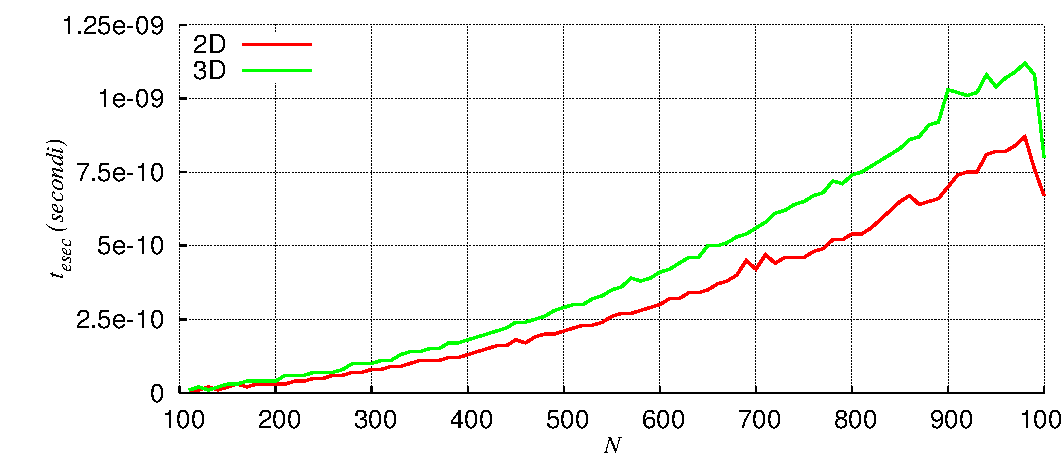
\includegraphics[scale=0.85]{Immagini/Soffici/TempoEsecuzione_ConfrontoD}

		\centering  \footnotesize{$\rho=0.8$ , Media su $ 1000000 $ passi}
	\end{figure}

Ovviamente si osserva un aumento del tempo-macchina con la crescita del numero di particelle simulate, questo determina un maggior numero test da effettuare per determinare la vicinanza tra le coppie .
\newline
D'altro canto una desità molto alta implica che le particelle siano statisticamente molto vicine tra loro, quindi, a parità del numero delle molecole, andranno calcolate in medeia le interazioni su un maggior numero di punti. Nella figura (\ref{fig: T_Esec_Confronto_rho Soffici}) è possibile osservare questo effetto.
\newline
La dimensionalità dello spazio influisce invece sul "impaccamento" delle particelle (soprattutto nelle configurazioni particolarmente dense). Ad esempio una sfera in uno spazio 3-dimensionale potrà venire a contatto con un maggiore numero di sfere sulla sua superficie rispetto ad un cerchio (quindi in 2 dimensioni) dello stesso raggio sulla sua superficie.
Il confronto tra i tempi di esecuzione tra  sistemi di dimensione diversa ma di pari densità è mostrato nella figura (\ref{fig: T_Esec_Confronto_D Soffici}).

	\begin{figure}[htbp]
		\centering
		\caption[Sfere Soffici$/$Preliminari\_TempoEsecuzione.cpp]{Confronto tra l'andamento del tempo di esecuzione a vari valori di densità del sistema.}\label{fig: T_Esec_Confronto_rho Soffici}\vspace{-15pt}
		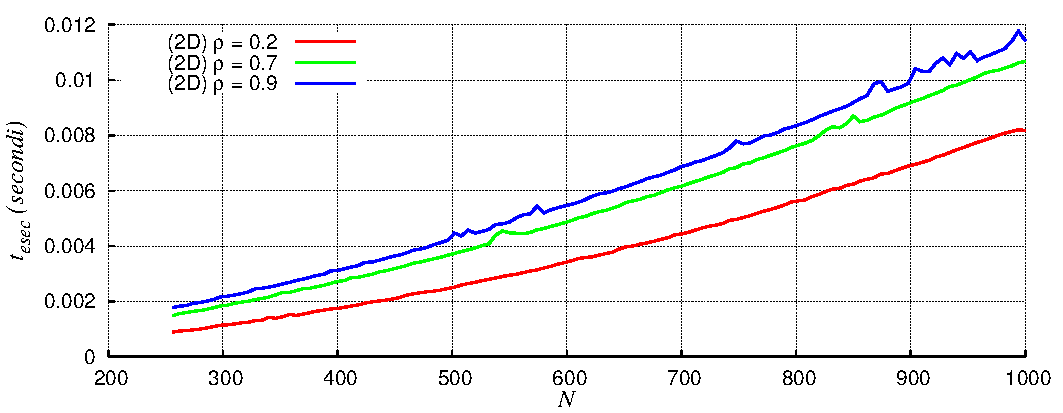
\includegraphics[scale=0.85]{Immagini/Soffici/TempoEsecuzione2D}

		\centering  \footnotesize{$d=2$ , Media su $ 50000 $ passi}
	\end{figure}


\FloatBarrier 
\subsubsection{Tempo di Termalizzazione}
In questo sistema è possibile definire due diversi processi di termalizzazione: nel primo si interviene fissando l'energia meccanica totale del sistema mentre nel seconda si fissa la temperatura del sistema, quindi solo l'enegia cinetica media.
Siccome le due quantità sono di natura differente, una è puramente istantanea e costantemente conservata mentre l'altra è una quantità soggetta a fluttuazioni termiche, lo studio del tempo di termalizzazione va effettuato in modo separato.

	\begin{figure}[htbp]
		\centering
		\caption[Sfere Soffici$/$Preliminari\_Termalizzazione.cpp]{Andamento degli osservabili istantanei in funzione del numero di passi d'evoluzione per vari valori di densità}\label{fig: Termal E D Soffici}\vspace{-15pt}

		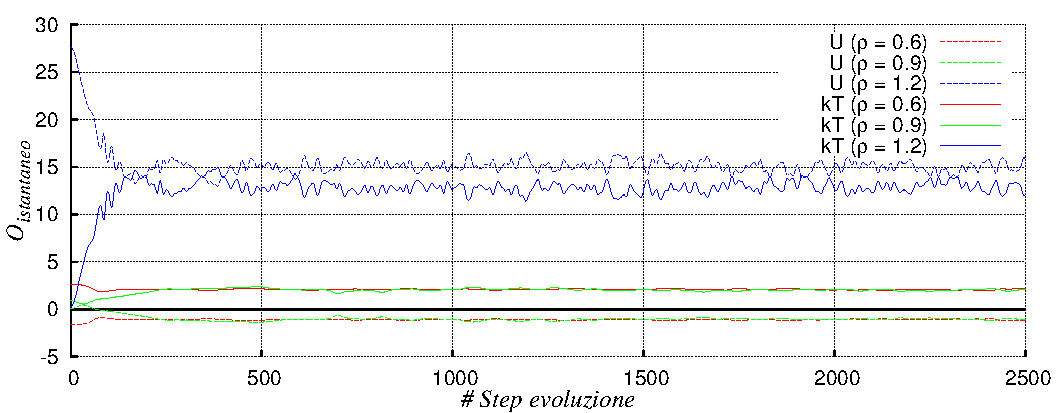
\includegraphics[scale=0.95]{Immagini/Soffici/Termal_OvsStep}

		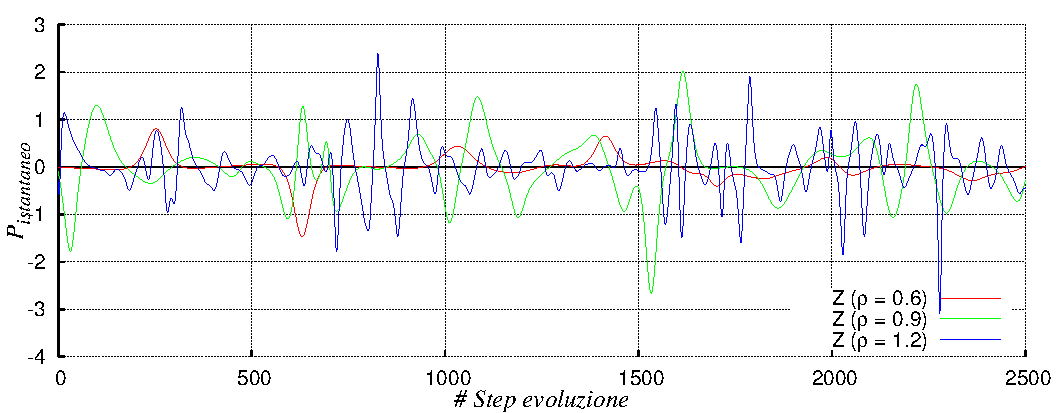
\includegraphics[scale=0.95]{Immagini/Soffici/Termal_PvsStep}

		\centering  \footnotesize{$N= 250$ , $d=3$ , $E_D$ per particella =1}
	\end{figure}
	
Il tempo di termalizzazione ad Energia definita si può studiare osservando l'andamento degli osservabili istantanei in funzione del numero di step di evoluzione, quando i valori tendono ad oscillare intorno ad un valore medio si può considerare raggiunta la condizione di termalizzazione. 
Secondo la figura (\ref{fig: Termal E D Soffici}) , dove è mostrato l'andamento di $P*$,$kT$ e$U$ in funzione del numero di passi di evoluzione, $500$ step sarebbero sufficienti a portare a termalizzazione un sistema di $250$ particelle.
\medskip\newline
Nel caso della termalizzazione a $kT$ definito, invece, è possibile sfruttare la funzione $H$ di Boltzman per valutare il tempo di termalizzazione.

	\begin{figure}[!htbp]
		\centering
		\caption[Sfere Soffici$/$Preliminari\_Termalizzazione.cpp]{Andamento dei valori della funzione di Boltzman in funzione del numero di passi d'evoluzione per vari valori di densità}\label{fig: Termal H T_D Soffici}\vspace{-15pt}
		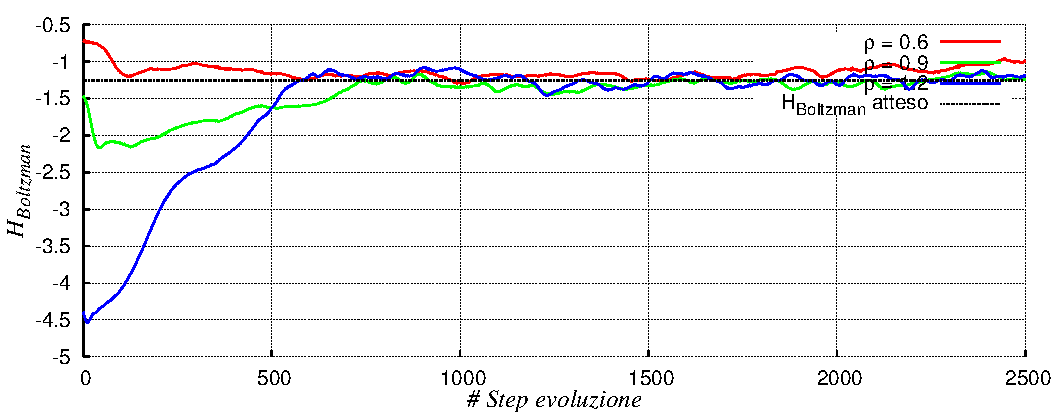
\includegraphics[scale=0.95]{Immagini/Soffici/Termal_HvsStep}

		\centering  \footnotesize{$N= 250$ , $d=3$ , $H$ media calcolata ogni 5 passi}
	\end{figure}
	
Nella figura (\ref{fig: Termal H T_D Soffici}) è mostrato l'andamento della funzione $H$ calcolata su $25$ configurazioni successive campionate dopo una termalizzazione a temperatura costante ( $kT=1$ ) effettuata per $n$ passi evolutivi a partire dal reticolo $BCC$ iniziale.
Dal grafico si può nota come i valori campionati comincino ad oscillare attorno al valore atteso dopo circa $1000$ evoluzioni, la statistica raccolta in un singolo istante non è sufficientemente ampia da poter approssimare l'istogramma delle componenti delle velocità alla loro effettiva distribuzione, in questo caso l'accordo completo non è mai raggiungibile.

	\begin{figure}[!htbp]
		\centering
		\caption[Sfere Soffici$/$Preliminari\_Termalizzazione.cpp]{Istogramma della distribuzione dei valori delle componenti x delle velocità raccolte dopo la termalizzazione}\label{fig: Termal Isto T_D Soffici}\vspace{-15pt}
		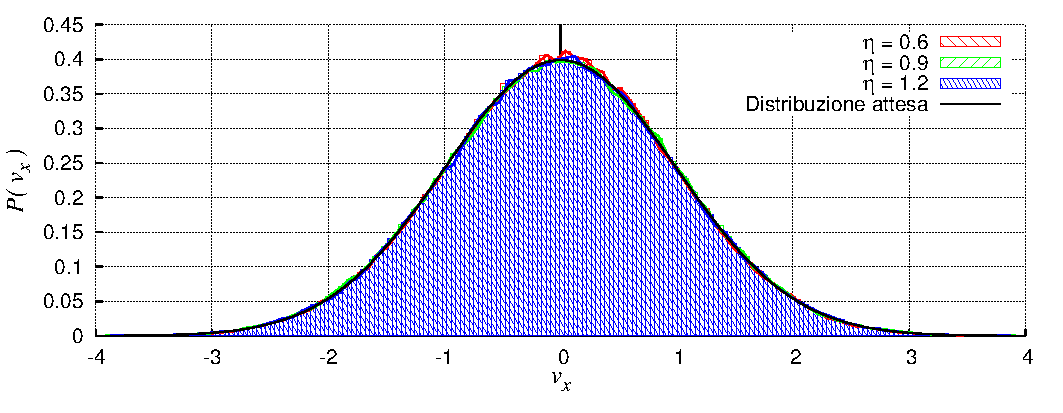
\includegraphics[scale=0.95]{Immagini/Soffici/DistroVx}

		\centering  \footnotesize{$N= 250$ , $d=3$ , N passi Termalizzazione =$ 5000$, $T_D=1$, intervallo di campionamento 50 step.}
	\end{figure}
	
Aumentando il numero di configurazioni campionate risulta, a seguito della termalizzazione precedente, la distribuzione di probabilità visibile in figura (\ref{fig: Termal Isto T_D Soffici}), che mostra un ottimo accordo con la distribuzione gaussiana prevista per la temperatura prescelta.


\FloatBarrier 
\subsection{Caratteristiche del modello, studio delle transizioni di fase}
In questo caso la determinazione della transizione di fase attraverso lo studio dell'andamento di un parametro d'ordine, quale Z, $ds^2$ o il numero medio di particelle vicini, è leggermente più impegnativa rispetto al modello precedente.

Il motivo di questa complicazione è da ricercare nella dipendenza dello stato non più dal solo parametro $\rho$ ma anche da $T_D$ che nel modello a sfere rigide era  una variabile fissata il cui valore determinava solamente un riscalamento dell'unità di tempo.
Per determinare la transizione di fase sarebbe necessario realizzare un grafico 3 dimensionale del parametro d'ordine in funzione delle due variabili di stato indipendenti. Tale procedimento è computazionalmente molto lungo in quanto richiederebbe il calcolo di troppi punti per ottenere una buona risoluzione, pertanto l'analisi della transizione di fase si limita allo studio della diffusione.


\subsubsection{Andamento delle Oscillazioni Termiche}
In un sistema conservativo l'energia meccanica totale è costantemente conservata ma in presenza, come in questo caso,  di un potenziale non nullo, non sono le singole componenti dell'energia ad essere conservate ma sono presenti continui scambi tra la componente interna e quella cinetica.
Nella figura (\ref{fig: Problema9}) è mostrata l'andamento della densità di energia interna istantanea, in un sistema già termalizzato, per due casi con diverso numero di particelle.

	\begin{figure}[htbp]
		\centering
		\caption[Sfere Soffici$/$Problema9.cpp]{Andamento dei valori della densità di energia interna istantanea in funzione del tempo di evoluzione a seguito della termalizzazione.}\label{fig: Problema9}\vspace{-15pt}

		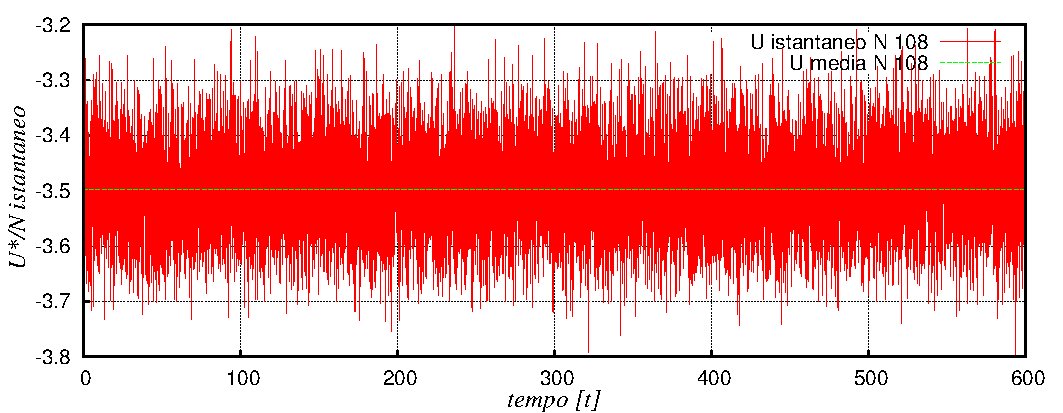
\includegraphics[scale=0.75]{Immagini/Soffici/UvsStepN108}

		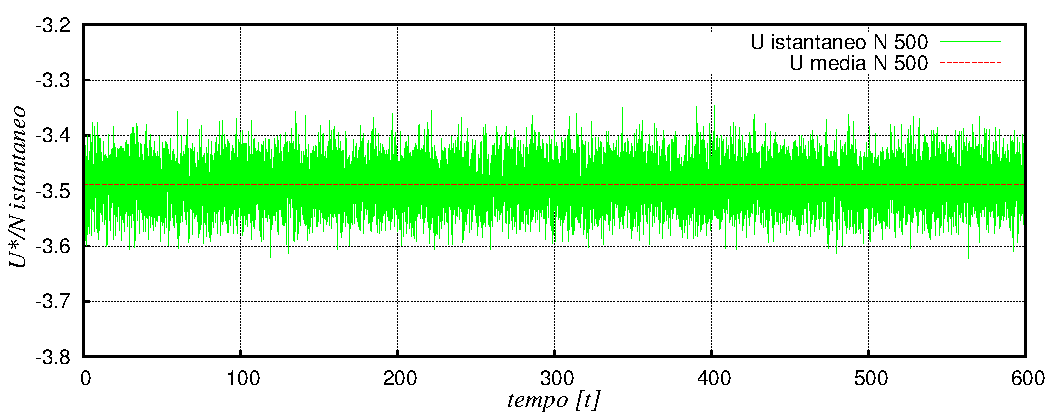
\includegraphics[scale=0.75]{Immagini/Soffici/UvsStepN500}

		\centering  \footnotesize{$N= 250$ , $d=3$ , N passi Termalizzazione =$ 5000$, $\rho = 0.7$,	$T_D=1.19$, campionamento ogni $0.015 [t]$.}
	\end{figure}

E' evidente come l'ampiezza delle fluttuazioni decresca all'aumentare del numero di molecole simulate (per conferma è stato realizzato nella figura (\ref{fig: Isto_Problema9}) l'istogramma dei valori istantanei raccolti), ci si aspetta che nel limite termodinamico tale quantità possa essere considerata una costante per un sistema in equilibrio.

	\begin{figure}[htbp]
			\centering
		\caption[Sfere Soffici$/$Problema9.cpp]{Istogramma dei valori campionati per la figura precedente.}\label{fig: Isto_Problema9}\vspace{-15pt}

		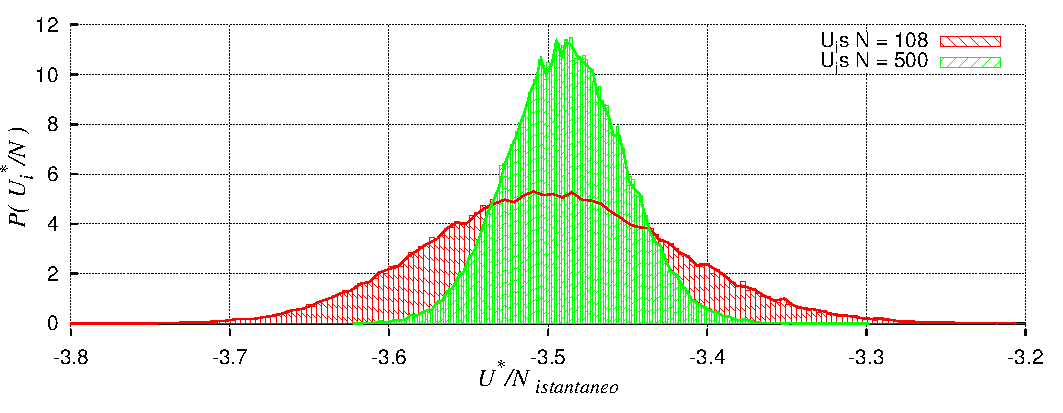
\includegraphics[scale=0.85]{Immagini/Soffici/IstoU}

	\end{figure}
	
Nella figura (\ref{fig: Problema10}) viene comparato l'andamento dei 3 osservabili istantanei in funzioni dei passi evolutivi. La prima prima cosa che si può notare è come la temperatura, legata all'energia cinetica media, oscilli in senso opposto rispetto alla densità di energia interna. L'effetto è dovuto alla conservazione dell'energia totale che obbliga le fluttuazioni ad annullarsi.
In secondo luogo, analizzando l'istogramma, si osserva che le oscillazione dell'osservabile $P*$ sono molto più ampie rispetto a quelle degli altri due.
	
	\begin{figure}[htbp]
		\centering
		\caption[Sfere Soffici$/$Problema10.cpp]{Andamento delle osservabili istantanee della simulazione in funzione del tempo di evoluzione a seguito della termalizzazione.}\label{fig: Problema10}\vspace{-15pt}
		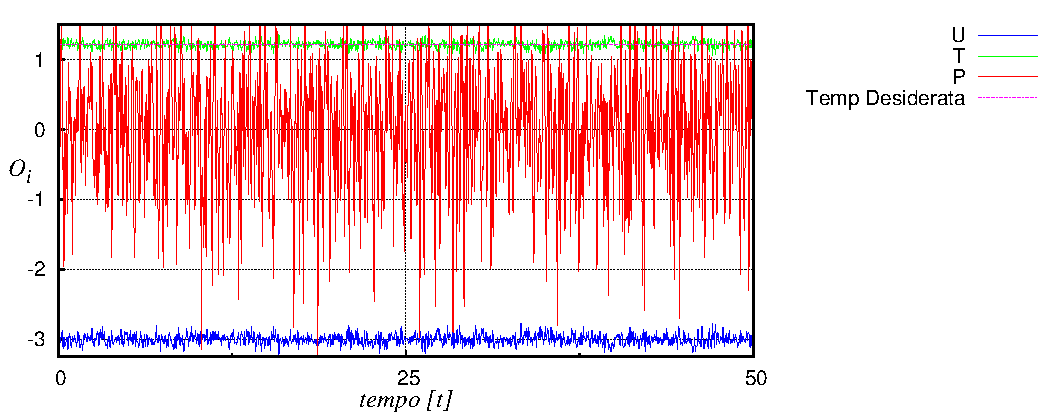
\includegraphics[scale=0.85]{Immagini/Soffici/OvsStep}

		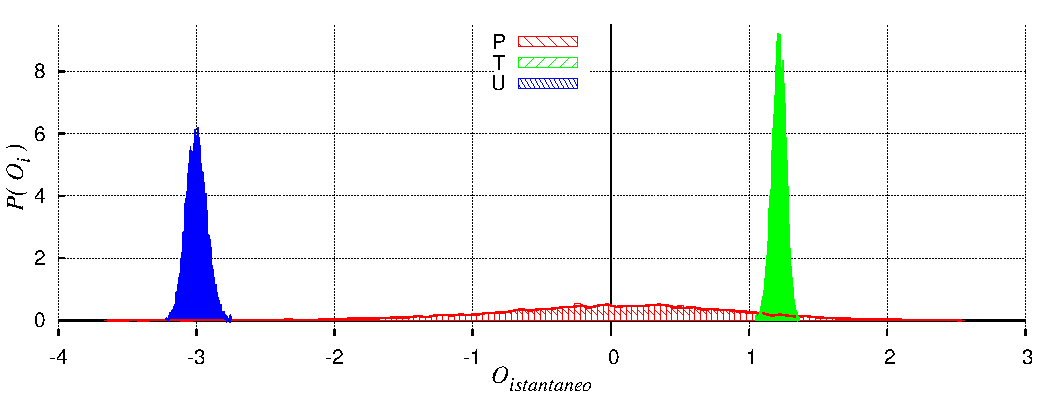
\includegraphics[scale=0.85]{Immagini/Soffici/IstoO}


		\centering  \footnotesize{$N= 108$ , $d=3$ , N passi Termalizzazione =$ 5000$, $\rho = 0.6$,	$T_D=1.22$, campionamento ogni $0.015 [t]$.}
	\end{figure}



\FloatBarrier 
\subsubsection{Studio della Diffusione: Spostamento Quadratico Medio e Funzione di Distribuzione Radiale}
Si procede ora allo studio della diffusione per determinare la fase fisica del sistema come spiegato nel capitolo introduttivo.

Nel grafico (\ref{fig: Problema11}) è mostrato l'andamento dello spostamento quadratico medio (calcolato senza bordo) in fuzione del tempo per lo stesso sistema a diverse temperature.
	\begin{figure}[htbp]
		\centering
		\caption[Sfere Soffici$/$Problema11.cpp]{Andamento dello spostamento quadratico medio in funzione del tempo di diffusione per vari valori di temperatura}\label{fig: Problema11}\vspace{-15pt}

		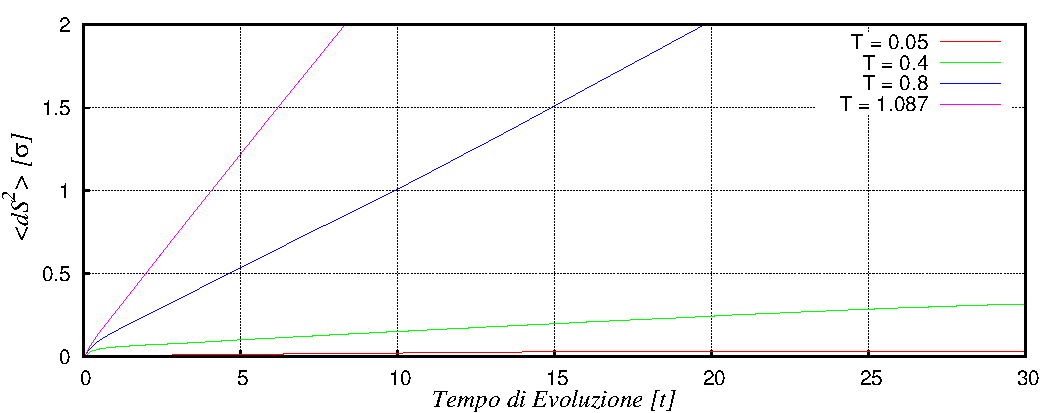
\includegraphics[scale=0.95]{Immagini/Soffici/dS_quadvsDt}

		\centering  \footnotesize{$N= 256$ , $d=3$ , N passi Termalizzazione =$ 10000$, $\rho = 0.9$, $\#$ campionature = $ 4000$, campionamento ogni $0.015 [t]$.}
	\end{figure}
Le simulazioni sono ottenute in modo consecutivo partendo dalla temperatura più bassa e termalizzando a temperature crescente per ottenere i diversi andamenti.


	\begin{figure}[htbp]
		\centering
		\caption[Sfere Soffici$/$Problema11$\_$v2C.cpp]{Funzione di distribuzione radiale $g_t(r)$ a vari valori di densità e temperatura alta.}\label{fig: Problema11_v2C}\vspace{-15pt}

		\includegraphics[scale=0.95]{Immagini/Soffici/DistrodS_RhoAlta_3D}
		
		\centering  \footnotesize{$N= 256$ , $d=3$ , N passi Termalizzazione =$ 10000$, $\rho = 0.9$, $\#$ campionature = $ 4000$,\newline $\Delta t = 0.015 [t] = 15 t_{step}$, intervallo di tempo tra ogni campionamento = 10 $\Delta t$, tempo di diffusione = 3000 $\Delta t$}
	\end{figure}
Calcolando la funzione di distribuzione radiale  per gli stessi sistemi si ottiene la figura (\ref{fig: Problema11_v2C}). E' evidente come alla temperatura $T=1.087$ il sistema si trovi in una fase liquida  mentre per la temperatura più bassa ($T=0.8$) sviluppi una struttura solida metastabile. In quest'ultimo caso sono visibili due picchi compatibili con la presenza simultanea di un nucleo denso localizzato, in grado di tratenere le particelle più lente, e un gas di particelle più veloci che riescono ad evaporare dall' aggregato congelato.
\medskip

Confrontando il sistema precedente con una simulazione dello stesso tipo ma a densità minore si può notare come la temperatura di cambiamento di fase sia determinata dalla velocità.
	\begin{figure}[htbp]
		\centering
		\caption[Sfere Soffici$/$Problema11$\_$v2B.cpp]{Funzione di distribuzione radiale $g_t(r)$ a vari valori di temperatura a partire dalla configurazione iniziale congelata a bassa densità.}\label{fig: Problema11_v2B}\vspace{-15pt}

		\includegraphics[scale=0.95]{Immagini/Soffici/DistrodS_RhoBassa_3D}

		\centering  \footnotesize{$N= 256$ , $d=3$ , N passi Termalizzazione =$ 10000$, $\rho = 0.25$, $\#$ campionature = $ 2000$,\newline $\Delta t = 0.05 [t] = 15 t_{step}$, intervallo di tempo tra ogni campionamento = 10 $\Delta t$, tempo di diffusione = 3000 $\Delta t$}
	\end{figure}
Nella figura (\ref{fig: Problema11_v2B}), in cui è rappresenatata la funzione di distribuzione radiale per un sistemà a densità  $\rho = 0.25$, si può notare come a temperature simili alla fase solida metastabile del sistema precedente il sistema a bassa densità si trovi già allo stato liquido. In questo caso, per eliminare il tempo  di evoluzione necessario al configurazione in disposizione $BCC$ di nucleare, il sistema è stato inizializzato già aggregato.

\medskip

Può essere interessante studiare la funzione $g_t(r)$ anche per sistema alla stessa temperatura ma con diversa densità.
Nella figura (\ref{fig: Problema11_v2A}) sono mostrati tali andamenti, si può vedere come il sistema possa termalizzarsi in uno stato solido anche a temperature alte se la densità è sufficientemente elevata.
	\begin{figure}[htbp]
		\centering
		\caption[Sfere Soffici$/$Problema11$\_$v2A.cpp]{Funzione di distribuzione radiale $g_t(r)$ a vari valori di densità e temperatura fissata.}\label{fig: Problema11_v2A}\vspace{-15pt}

		\includegraphics[scale=0.95]{Immagini/Soffici/DistrodS_Rho_3D}
		
		\centering  \footnotesize{$N= 256$ , $d=3$ , N passi Termalizzazione =$ 10000$, $T_D = 0.9$, $\#$ campionature = $ 2000$,\newline $\Delta t = 0.05 [t] = 15 t_{step}$, intervallo di tempo tra ogni campionamento = 10 $\Delta t$, tempo di diffusione = $3000 Delta t$}
	\end{figure}



\FloatBarrier 
\subsection{Studio del limite termodinamico}
Si procede ora alla stima dei variabili di stato di un sistema al limite termodinamico. Nella figura (\ref{fig: Limite Termo}) è mostrato il valore di $\langle Z-1 \rangle$  calcolato per sistemi caratterizzati dalla stessa densità ed energia molecolare media ma simulati con diverso numero di particelle.

\begin{figure}[htbp]
\centering
	\caption[Sfere Soffici$/$Problema12.cpp $\quad \rightarrow \quad$ ZvsN\_file.p]{Andamento del parametro Z-1 in funzione di $N$. Limite Termodinamico }\vspace{-15pt}
	\includegraphics[scale=0.95]{Immagini/Soffici/ZvsN3D}
	\newline\footnotesize{ $d=3$ , campioni$= 500000$,  urti termal=$ 250000$, $\rho = 0.7$,	$E_D=-2.98$ per molecola}
	\label{fig: Limite Termo}
\end{figure}

Eseguendo un fit dei valori calcolato rispetto ad un andamento del tipo:
\begin{equation}\label{eq: limiteTermo}
 (Z-1) = A + \dfrac{B}{N}
\end{equation}
si ottengono le seguenti stime per i parametri della funzione:
\begin{center}
\begin{tabular}{|c c r c l |}
\hline
	A	 & $=$ & $ 2.98 $ & $\pm$ & $0.01 $	\\
	B	 & $=$ & $ 2.70$ & $\pm$ & $0.2 $	\\
\hline
\end{tabular}
\end{center}

Calcolando il limite per $N\rightarrow \infty$ si ottiene una stima del fattore di comprimibilità al limite termodinamico (a densità $\rho=0.7$ ed energia molecolare media $E_{mol} = -2.98$) pari a: 
\begin{displaymath}
Z_{\textrm{TD}} = 1 \pm 0.0001
\end{displaymath}

Un valore di Z pari ad 1 implica che il sistema in questo stato termodinamico soddisfa approsimativamente l'equazione di stato dei gas Perfetti:
\begin{displaymath}
 P V = n R T \rightarrow 1= \dfrac{P V}{n R T} =\dfrac{P \rho}{kT} = Z
\end{displaymath}
\newline \bigskip
Con lo stesso sistema è possibile studiare il limite termodinamico anche per gli altri osservabili del sistema.
Nella figura (\ref{fig: Limite Termo T}) è mostrato l'andamento di $T$ mentre nella figura (\ref{fig: Limite Termo U}) quello di $\frac{U}{N}$ espressi nelle unità dimensionali del modello e in funzione del numero di molecole $N$.
\begin{figure}[htbp]
\centering
	\caption[Sfere Soffici$/$Problema12.cpp $\quad \rightarrow \quad$ UvsN\_file.p]{Andamento dell'osservabile $\lbrace U/N \rbrace$ in funzione di $N$. Limite Termodinamico }\vspace{-15pt}
	\includegraphics[scale=0.95]{Immagini/Soffici/UvsN3D}
	\newline\footnotesize{ $d=3$ , campioni$= 500000$,  urti termal=$ 250000$, $\rho = 0.7$,	$E_D=-2.98$ per molecola}	\label{fig: Limite Termo U}
\end{figure}
\begin{figure}[htbp]
\centering
	\caption[Sfere Soffici$/$Problema12.cpp $\quad \rightarrow \quad$ TvsN\_file.p]{Andamento del parametro $\lbrace T \rbrace$ in funzione di $N$. Limite Termodinamico }\vspace{-15pt}
	\includegraphics[scale=0.95]{Immagini/Soffici/TvsN3D}
	\newline\footnotesize{ $d=3$ , campioni$= 500000$,  urti termal=$ 250000$, $\rho = 0.7$,	$E_D=-2.98$ per molecola}	\label{fig: Limite Termo T}
\end{figure}
Usando per il fit di queste osservabili l'andamento precedente ( equazione \ref{eq: limiteTermo}) risulta la seguente stima per il limite termodinamico della temperatura e dell'energia interna:
\begin{displaymath}
T_{\textrm{TD}} = 0.6214 \pm 0.0003
\end{displaymath}
\begin{displaymath}
(U/N)_{\textrm{TD}} = -3.912 \pm 0.0005
\end{displaymath}
Si può osservare che i valori soddisfano la prescrizione di conservazione dell'energia meccanica totale:
\begin{displaymath}
\lbrace T \rbrace \dfrac{3}{2} + \lbrace U/N \rbrace =  0.931 - 3.912 = -2.98
\end{displaymath}

\FloatBarrier
\listoffigures

\bibliographystyle{plain}
\bibliography{Bibi.bib}


\end{document}
This is never printed


classi \Cls{Nomeclasse}

metodi \cd{NomeMetodo}

tipo \cd{Nometipo}
